% Apostel, Bogdanski, Ritter
%
% Wahlpflichtfach Künstliche Intelligenz:
% Projekt - Schiffe Versenken
%
% Hochschule Bremen - University of applied siences
% ============================================================================
%
% report.tex
%
% das Wurzel-Dokument, fügt alle einzelteile zusammen

%!TEX root = /Users/stefanbogdanski/Dropbox/BÄTTLESHÖP/Dokumentation/dokumentation.text
% 
% Apostel, Bogdanski, Ritter
%
% Wahlpflichtfach Künstliche Intelligenz:
% Projekt - Schiffe Versenken
%
% Hochschule Bremen - University of applied siences
% ============================================================================
%
% header.tex
%
% Präambel und LaTeX Einstellungen

\documentclass[
    pdflatex,           % Use PDFTex
    a4paper,            % A4 paper
    oneside,            % oneside print
    12pt,               % Font size 12pt
    captions=tableheading,  % korrekte Abstaende bei TabellenUEBERschriften
    chapterprefix,      % Chapter write to as chapter
    headsepline,        % Line after header
    footsepline,        % Line before footer
    headinclude,        % Kopfzeile wird Seiten-Layouts mit beruecksichtigt
    footinclude=false,  % Fu{\ss}zeile wird Seiten-Layouts mit 
    plainheadsepline,   % horizontale Linie auch beim plain-Style
    fleqn,              % Write the formula left-aligned
    appendixprefix,
	bibtotocnumbered,	%referencen mit nummerieren und ins inhalts VZ 
	dvipsnames
]{scrartcl}
\usepackage{graphicx}
\usepackage{graphics}
\usepackage{epsf}
\usepackage{epsfig}
\usepackage{amsmath}
%
% package for the appendix.
%
\usepackage{appendix}

% mehrzeilige Captions ausrichten
\usepackage[font=footnotesize]{caption}
%
% package to create subfigure, subtables
%
\usepackage{subfigure} 

%
%package to include pdf-files to Latex Document
%
\usepackage{pdfpages}

%
% package for the index.
%
\usepackage{makeidx} 

\usepackage{rotfloat}



%
% using babel
%
\usepackage[ngerman]{babel}

%
% package to use the UTF8 character and their writings
%
\usepackage[utf8]{inputenc}
%\usepackage[T1]{fontenc}
\usepackage{textcomp}

%
% Flie{\ss}umgebung: Erm\"{o}glicht Platzierung [H] f\"{u}r Grafiken und Tabellen
%
\usepackage{float}
\restylefloat{figure}
\restylefloat{table}

%
% package for more table settings
%
\usepackage{array}%,tabularx}
%\usepackage[table,svgnames]{xcolor}
\usepackage{ragged2e}

\usepackage{setspace}            % Zeilenabstand einstellbar
\onehalfspacing                  % eineinhalbzeilig einstellen

\typearea[current]{current}        % Neuberechnung des Satzspiegels mit alten Werten nach \"{A}nderung von Zeilenabstand,etc


%
% header und footer
%
%\pagestyle{headings}
%\usepackage{scrpage2}            % Kopf und Fusszeilen-Layout
\renewcommand{\headfont}{\normalfont\sffamily}    % Kolumnentitel serifenlos
\renewcommand{\pnumfont}{\normalfont\sffamily}    % Seitennummern serifenlos
%\pagestyle{headings}
%\ihead[]{\headmark}              % Kolumnentitel immer oben innen
%\ohead[\pagemark]{\pagemark}     % Seitennummern immer oben aussen
%\ofoot{\pagemark}                       % Seitennummern in der Fusszeile loeschen

\usepackage[automark]{scrpage2}
\ihead{}
\ohead{\headmark}
\chead{}
\cfoot{}
\ofoot{\pagemark}

\pagestyle{scrheadings}

% 
\usepackage{blindtext}
% define the color "LinkColor"
%
\definecolor{LinkColor}{rgb}{1,0,0}
\definecolor{CiteColor}{rgb}{0,1,0}
\definecolor{URLColor}{rgb}{0,0,1}

%
% package for using Hyperlinks in PDF files
%
 \usepackage[
	pdftitle={Projekt - Schiffe Versenken},
	pdfauthor={Apostel, Bogdanski, Ritter},
	pdfsubject={Wahlpflichtfach KI},
	plainpages=true
    ]{hyperref}
\hypersetup{colorlinks=false,
	linkcolor=LinkColor,
	citecolor=CiteColor,
	filecolor=LinkColor,
	menucolor=LinkColor,
%	pagecolor=LinkColor,
	urlcolor=URLColor}

%
% package to represent listings in their formats
%

\usepackage[colorinlistoftodos]{todonotes}
\newcommand{\todoin}[1]{\todo[inline]{#1}}

%
% package to use the abstract environment
%
\usepackage{abstract}

%
% package to use URLs
%
\usepackage{url}
\usepackage{listings} 
%\usepackage{color} 
%\usepackage[dvipsnames]{xcolor}  

%
% build index
%
\makeindex

%
% build glossary
%
\makeglossary

%\usepackage[savemem]{listings}


\usepackage{longtable}

\begin{document}
	\listoftodos
	\pagenumbering{Alph}
		%!TEX root = /Users/stefanbogdanski/Dropbox/BÄTTLESHÖP/Dokumentation/dokumentation.tex
%
% Apostel, Bogdanski, Ritter
%
% Wahlpflichtfach Künstliche Intelligenz:
% Projekt - Schiffe Versenken
%
% Hochschule Bremen - University of applied siences
% ============================================================================
%
% 0_deckblatt.tex
%
% Beschreibung des Dateiinhalts
\begin{titlepage}
	\begin{figure}[lt] % (fold)
		
\includegraphics[scale=0.5]{images/logo_a4.pdf}
	\end{figure}
	% figure figure label (end)
	\begin{Center}
		\Huge
		Wahlpflichtfach KI\newline
		\vspace*{1cm}
		\Large
		Projektdokumentation: Schiffe Versenken
	\end{Center}	
	\vfill
	\begin{table}[H] % (fold)
		\centering
		\begin{tabular}{ll}
			Autoren: & Victor Apostel, Stefan Bogdanski, Sibille Ritter \\
			Studiengang: & (Internationaler) Studiengang Technische Informatik B.Sc. \\
		\end{tabular}
		\label{label}
	\end{table}
	\todoin {Liebe Gruppenmitglieder, \newline so langsam müssen wir auch bedenken, dass dieses Dokument nicht den Rahmen sprengen darf. m.E. ist es bereits viel zu lang! Der Inhalt ist - wie zu erwarten - auf einem sehr schönen qualitativen Niveau. Aber man darf es hier nicht aus den Fugen laufen lassen. Denkt daran, dass der 'arme' Prof. Breymann das auch alles lesen muss. Wir haben inzwischen ein fast 40(!!!) seitiges Pamphlet zu einer Implementierung von Schiffe versenken verfasst.\newline Ich bin mir bewusst, dass mein Anteil an diesem Dokument der geringste ist, und ich will mich bei Leibe nicht darüber beschweren, dass soviel von euch geschrieben wurde! Aber trotzdem möchte ich apellieren, dass der Rahmen m.E. bereits überschritten ist und nun die Zeit gekommen ist auf die bremse zu treten. Dies ist keine Bachelor-Thesis, dies ist ein WPM. LG, HEGDL und alles! - SB}
\end{titlepage}
	\pagenumbering{roman}
		%\include{chapters/02_abstract}
	\pagenumbering{arabic}
		%!TEX root = /Users/stefanbogdanski/Dropbox/BÄTTLESHÖP/Dokumentation/dokumentation.text
% 
% Apostel, Bogdanski, Ritter
%
% Wahlpflichtfach Künstliche Intelligenz:
% Projekt - Schiffe Versenken
%
% Hochschule Bremen - University of applied siences
% ============================================================================
%
% toc.tex
%
% Generiert das Inhaltsverzeichnis
\tableofcontents
		\listoffigures 
		\listoftables
		\clearpage 
		%% Apostel, Bogdanski, Ritter
%
% Wahlpflichtfach Künstliche Intelligenz:
% Projekt - Schiffe Versenken
%
% Hochschule Bremen - University of applied siences
% ============================================================================
%
% 1_chapter.tex
%
% Beschreibung des Dateiinhalts
\section{Dummysection} % (fold)
\label{sec:dummysection}
	\blindtext
% section dummysection (end)
		\section{Einleitung}
\label{sec:Einleitung}
	\todoin {Sibille, bitte Rechtschreibung prüfen :-/ \newline Reicht das so!?}
	Im Wahlpflichtfach "'Künstliche Intelligenz"' wurde während der Vorlesungen, den Vorlesungsbegleitenden Beispielen 
	sowie in den Laboraufgaben ein solides Verständnis und Wissen über die Implementierung einer künstlichen Intelligenz 
	mithilfe der Programmiersprache "'Prolog"' erarbeitet. Zum Ende der Veranstaltung soll das angeeignete Wissen nun in 
	Form eines Projekts in Gruppenarbeit dargestellt und weiter vertieft werden.
	
	Die vorliegende Dokumentation beschreibt die Entwicklung des Spiels "'Schiffe-Versenken"' ("Battleship"), welches 
	mithilfe der Programmiersprachen Java und Prolog implementiert wird.
	
	Ziel des Projekts ist es das Spiel gegen den "'Computer"' spielen zu können. Hierfür muss das Spiel mit allen Spielregeln 
	in Prolog abgebildet werden. Ebenso muss eine Spielstrategie für den Computerspieler konzeptioniert und implementiert werden, 
	welche dafür sorgt das die künstliche Intelligenz Siegesorientiert spielt. 
	Eine Benutzungsfreundliche Oberfläche für menlische Spieler wird durch ein Java-Programm realisiert.
	
	\subsection{Anforderungen} % (fold)
	\label{sub:anforderungen}
		Von den Gruppenmitgliedern wurden die Folgenden Anforderungen für die Software definiert:
		\begin{itemize}
			\item Das Prolog Programm kommuniziert über Sockets mit der Java-Benutzerschnittstelle.
			\item Prolog-Implementierungen von Modulen zum Regeln des/der:
			\begin{itemize}
				\item generellen Spielablaufs,
				\item platzieren von Schiffen auf dem Spielfeld,
				\item Antworten auf "'Angriffe"',
				\item "'Angreifen"' des gegenspielers nach einer 
				\item Siegstrategie.
			\end{itemize}
			\item Es soll möglich sein, selbst gegen die künstliche Intelligenz zu spielen.
			\item Es soll möglich sein, dass zwei Instanzen der künstlichen Intelligenz eine bestimmte Anzahl von spielen gegeneinander 
			austragen.
		\end{itemize}
		Neben diesen Anforderungen ist eine weitere, spezielle, Anforderung definiert:
		
		Da eine weitere Gruppe von Studenten des Moduls ebenfalls das Spiel "'Schiffe-Versenken"' als Projektthema wählten, soll 
		es möglich sein, dass die künstlichen Intelligenzen beider Gruppen gegeneinander antreten können. 
		Hierfür ist die Abstimmung eines Protokolls zur Kommunikation mit der anderen Gruppe notwendig.
	% subsection anforderungen (end)
		\section{Spielregeln}
\label{sec:Spielregeln}

Im folgenden werde die Spielregeln des Spiels \emph{Schiffe-Versenken} beschrieben. Diese allgemein gültigen Regeln, sind für 
die im folgenden beschriebene Umsetzung des Spiels in Prolog und Java als Spezifikation anzusehen.

%Da die allgemeinen Regeln des Spiels \textit{Schiffe-Versenken} bekannt sein sollten, werden an dieser Stelle nur die relevanten Eckdaten 
%und besondere Vereinbarungen aufgeführt:

\todoin{Findet jemand Fehler, Mehrdeutigkeiten, Ungenauigkeiten, Auslassung?!- SB}

\begin{itemize}
	\item \textbf{Spielfeld} \newline Für das eigene und das gegnerische Spielfeld gelten die folgenden Regeln:
		\begin{itemize}
			\item Das Spielfeld eines jeden Spielers ist 10x10 Felder groß.
			\item Jedes eigene Feld hat einen der folgenden Status: Wasser, Schiff, Getroffen oder Versenkt
			\item Jedes gegnerische Feld hat infolgedessen einen der folgenden Status: Unbekannt, Wasser, Treffer oder Versenkt.
		\end{itemize}
	\item \textbf{Schiffe} \newline Für die am Spiel beteiligten Schiffe gelten die folgenden Regeln:
		\begin{itemize}
			\item Folgende Schiffe müssen auf dem Spielfeld platziert werden: 1x 5er, 1x 4er, 2x 3er, 1x 2er.
			\item Schiffe dürfen einander nicht berühren.
			\item Schiffe dürfen Horizontal und Vertikal, nicht aber Diagonal auf dem Spielfeld platziert werden. % Fragt sich, ob Sie AKTROPHAL positioniert werden können ;-) - kleiner Scherz ... höhö
			\item Schiffe dürfen Diagonal versetzt (Aneinander liegende Eckpunkte) platziert werden.
			\item Schiffe dürfen nach der ersten Platzierung nicht mehr verschoben werden.
		\end{itemize}
	\item \textbf{Spielablauf} \newline Für den Spielablauf gelten die Folgenden Regeln und abläufe:
		\begin{itemize}
			\item Beide Spieler 'schießen' abwechselnd auf das Spielfeld des anderen.
			\item Das Los entscheidet, welcher Spieler beginnt.
			\item Ein angreifender Spieler teilt dem Gegner die angegriffene Koordinate mit (bspw. "E5").
			\item Der angegriffene Spieler Antwortet nun wahrheitsgemäß mit:
				\begin{itemize}
					\item \emph{"Wasser!"} wenn kein Schiff auf dem angegriffenen Feld steht.
					\item \emph{"Treffer!"} wenn ein Schiff auf dem angegriffenen Feld steht.
					\item \emph{"Versenkt!"} wenn der letzte Teil eines Schiffes auf diesem Feld getroffen wurde.
				\end{itemize}
			\item \textbf{Spielende:} Es gewinnt der Spieler, der zuerst alle Fünf Schiffe des Gegners versenkt hat.
		\end{itemize}
\end{itemize}
		\section{Kommunikationsprotokoll}
\label{sec:Kommunikationsmodell}

Die Kommunikation zweier Spieler erfolgt auf Basis von Textnachrichten, den sogenannten Kommandos, die einer fest definierten Codierung genügen.
Das Ziel dieses Kapitels ist die Erläuterung des Nachrichtenaufbaus und deren Interpretation.

Jedes Kommando, das es zu interpretieren gilt, ist aus Gründen der Prologkompatibilität mit runden Klammern umgeben und endet mit einem "'."'.
Da zudem stets ganze Zeilen verarbeitet werden sollen, wird der Nachricht das nicht druckbare Zeichen "'\textbackslash n"' angehängt.
Damit wird signalisiert, dass die gesamte Nachricht übermittelt wurde.

Innerhalb der umschließenden runden Klammern werden zwei Angaben erwartet.
Die erste Angabe wird als \emph{Opcode} bezeichnet und dient der eindeutigen Bestimmung des Kommandotyps.
Die zweite Angabe des Kommandos ist eine, von eckigen Klammern umgebene Parameterliste und kann null bis drei, durch Kommata getrennte, nummerische Elemente beinhalten.
Die Anzahl der erwarteten Parameter richtet sich nach dem übermittelten Opcode.

Die formale Beschreibung des Kommandoaufbaus liegt im Folgenden in Form von regulären Ausdrücken vor.

\begin{align*}
	COMMAND &:= \text{\textbackslash}(OPCODE,LIST\text{\textbackslash}) \text{\textbackslash}. NEWLINE \\
	LIST &:= \text{\textbackslash}[ [PARAMS]? \text{\textbackslash}] \\
	NEWLINE &:= \text{\textbackslash \textbackslash} r \\
	OPCODE &:= [1-5] \\
	PARAMS &:= [0-9]+[,[0-9]+]\{0,2\}
\end{align*}

Der Spielablauf durchläuft mehrere Zustände, die durch das Kommunikationsprotokoll abgedeckt werden müssen.
So startet jeder Spieler in einem Initialisierungszustand.
In diesem Zustand wird festgelegt, welcher der beiden Spieler den ersten Angriff ausführt.

\todoin{Da wird plötzlich vom Server angefangen, ohne jemals erwähnt zu haben, dass wir einen haben! Den Absatz vllt in eine Server - section packen?}
Stellt der Server eine gültige Anzahl an verbundenen Spielteilnehmern fest, sendet dieser ein Startsignal an alle Teilnehmer und die Clients wechseln ihrerseits vom Initialisierungszustand in den Angriffs-, bzw. Verteidigungszustand.
Weitere Nachrichten die es zu übertragen gilt, sind zum Einen der Angriff auf eine Feldkoordinate, sowie zum Anderen das Ergebnis des Angriffs.

Die Abbildung der genannten Aktionen in Opcodes, sowie die erwarteten Parameter können der Tabelle \ref{tbl:Kommunikationsprotokoll} entnommen werden.

\begin{table}[H]
	\centering
	\begin{tabular}{|c|l|c|c|c|}
		\hline
		\textbf{Opcode}	&	\textbf{Bedeutung}	&	\textbf{Param 1}	&	\textbf{Param 2}	&	\textbf{Param 3} \\
		\hline
		\hline
		1				&	Angriff				&	X						&	Y				&	-	\\
		\hline
		2				&	Ergebnis des Angriffs	&	X					&	Y				&	Ergebnis	\\
		\hline
		3				&	Spieler startet im Verteidigungszustand	&	-	&	-				&	-	\\
		\hline
		4				&	Spieler startet im Angriffszustand	&	-		&	-				&	-	\\
		\hline
		5				&	Startsignal			&	-						&	-				&	-	\\
		\hline
	\end{tabular}
	\caption{Kommunikationsprotokoll}
	\label{tbl:Kommunikationsprotokoll}
\end{table}

Das Ergebnis eines Angriffs wird ebenfalls kodiert übertragen und kann den Zustand des Clients beeinflussen.
Im Regelfall sendet bzw. empfängt dieser die Ereignisse "'Wasser"', "'Schiff wurde getroffen"', oder "'Schiff wurde versenkt"'.
Des Weiteren kann als Reaktion auf einen Angriff die Nachricht eintreffen, dass das letzte Schiff versenkt wurde.
In diesem Fall wechseln die Clientzustände in Abhängigkeit vom Sender und Empfänder dieser Nachricht in "'gewonnen"' bzw. "'verloren"'.

Eine Auflistung der möglichen Ergebnisse eines Angriffs ist in Tabelle \ref{tbl:Ergebniskodierung} gegeben.

\begin{table}[H]
	\centering
	\begin{tabular}{|c|l|c|c|c|}
		\hline
		\textbf{Code}	&	\textbf{Bedeutung} \\
		\hline
		\hline
		1				&	Wasser	\\
		\hline
		2				&	Schiff wurde getroffen	\\
		\hline
		3				&	Schiff wurde getroffen und versenkt	\\
		\hline
		4				&	Letztes Schiff wurde versenkt. Das Spiel ist beendet	\\
		\hline
	\end{tabular}
	\caption{Ergebniskodierung}
	\label{tbl:Ergebniskodierung}
\end{table}

		\section{Softwarearchitektur} \label{sec:Softwarearchitektur}

\todoin{Beschreibung der Schnittstellen, z.B. Dateien und ihre Struktur, Benutzte Module/Bausteine und ihre Einbindung, Installationsvorschriften}

Die Software des Spiels "'Schiffe versenken"' wurde als Client-Server Anwendung gemäß Abbildung \ref{fig:Kommunikationsteilnehmer} entworfen.
Die zentrale Kommunikationsschnittstelle stellt der Kommunikationsserver dar, der auf dem Port $54321$ eingehende Verbindungen annimmt.
Verbindungen können sowohl mittels eines Java-Clients hergestellt werden, die von einem Menschen bedient werden, als auch von Prolog-Clients, die vollständig autonom agieren.
Es liegen hinsichtlich der Clientkombinationen keine Beschränkungen vor, sodass auch z.B. ein Prolog-Client gegen einen anderen Prolog-Client antreten kann.

\begin{figure}[H]
  \centering
  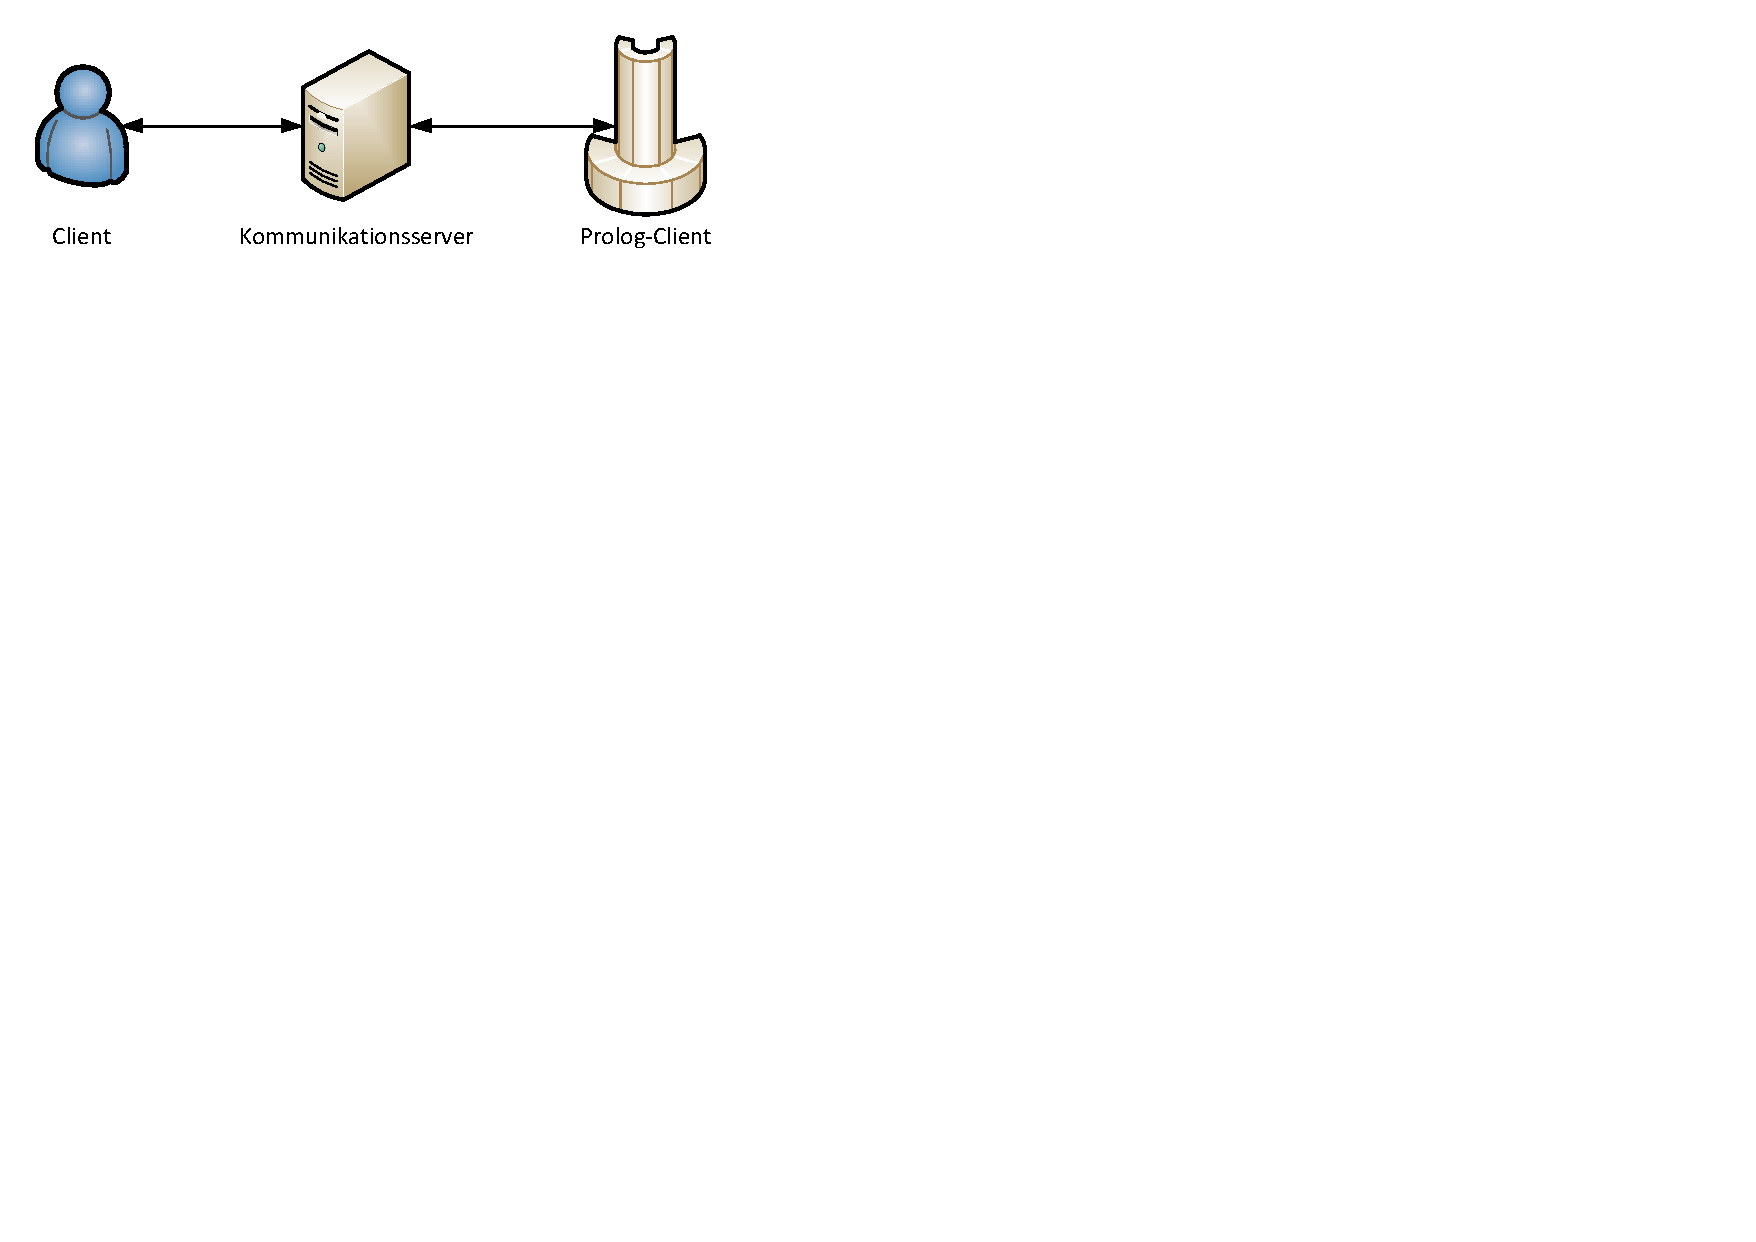
\includegraphics[trim=0mm 165mm 175mm 0mm,clip,width=0.5\textwidth]{images/Kommunikationsmodell.pdf}
  \caption{Darstellung der möglichen Kommunikationsteilnehmer}
  \label{fig:Kommunikationsteilnehmer}
\end{figure}

Der gesamte Spielverlauf lässt sich anhand der Statusdiagramme in den Abbildungen \ref{fig:Clientstates} und \ref{fig:SubClientstates} beschreiben.
Diese sind sowohl für den Javaclient, als auch für das Prologprogramm gültig.

Unmittelbar nach Start des Clients befindet sich dieser im Initialisierungszustand \emph{INITIALIZATION}.
Während dieser Phase obliegt es dem Client seine Schiffe gemäß den Regeln zu platzieren.
Des Weiteren hat er eine Nachricht des Servers zu empfangen, die angibt, ob sein initialer Zustand \emph{DEFENCE} oder \emph{ATTACK} sein soll, wenn er in die \emph{RUNNING}-Phase übergeht.
Dieser Übergang erfolgt durch den Empfang des Startkommandos, mit dem Opcode = 5.

\begin{figure}[H]
  \centering
  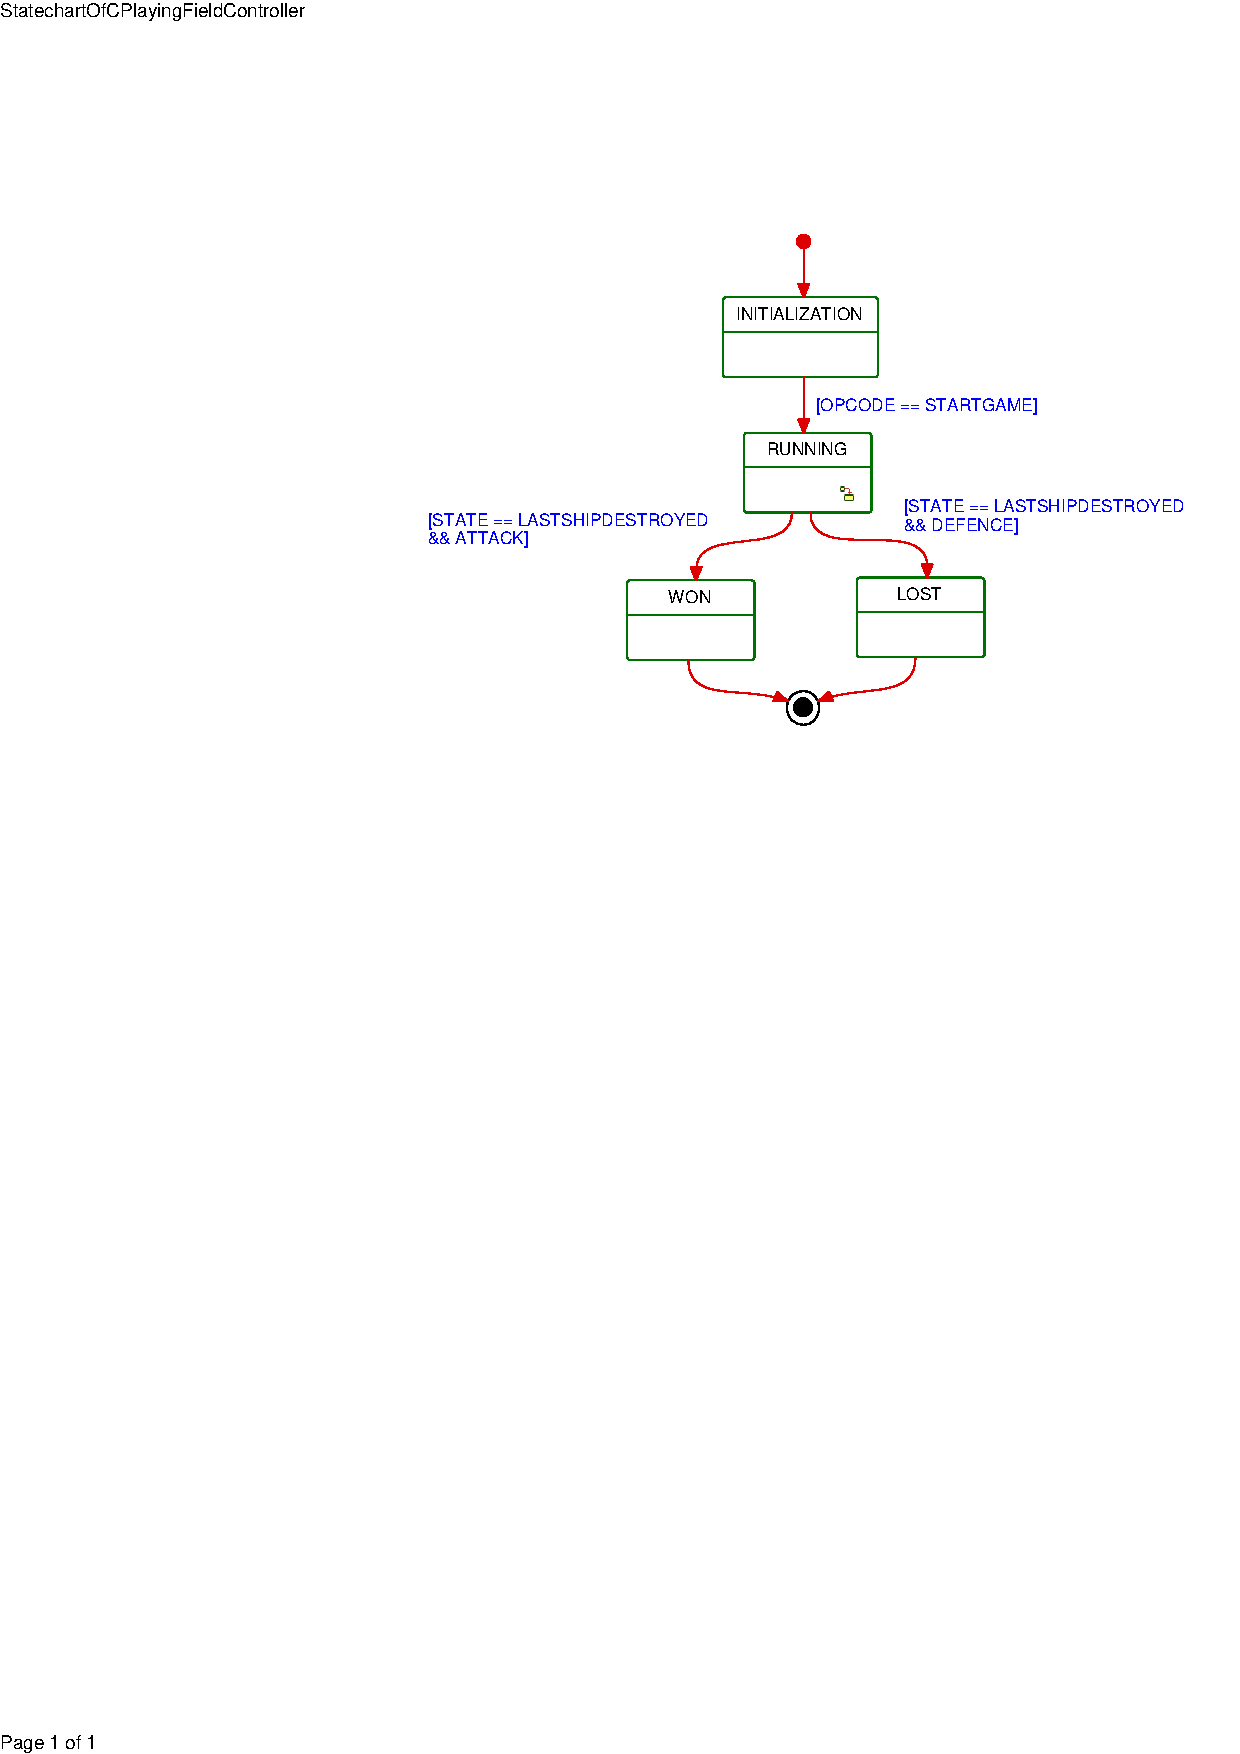
\includegraphics[trim=70mm 170mm 5mm 39mm,clip,width=0.7\textwidth]{images/SMController.pdf}
  \caption{Zustandsübergänge des Clients}
  \label{fig:Clientstates}
\end{figure}

%\todoin{Vic - Bemerkung zur Grafik: es gibt doch garkeinen OPCODE == LOST oder WON? Meiner Meinung nach wird der Zustandsübergang wird durch 'letztes Schiff versenkt' ausgelöst und dann hängt es davon ab, ob es das eigene ist oder nicht..? gleiches gilt für die folgende abbildung}

Befindet sich der Client im \emph{RUNNING}-Status, so wechselt er zwischen seinen internen Zuständen \emph{ATTACK} und \emph{DEFENCE} hin und her.
Dieser Wechsel erfolgt immer dann, wenn eine \emph{ATTACKRESPONSE} Nachricht mit dem Opcode = 2 übertragen wurde.
Der primäre Unterschied zwischen beiden Zuständen ist die Reihenfolge der erwarteten Nachrichten.
Befindet sich der Client im Subzustand \emph{DEFENCE}, so erwartet er von seinem Kontrahenten eine Nachricht mit dem Opcode = 1 und beantwortet diese seinerseits mit dem Opcode = 2.
Sollte sich der Client im Subzustand \emph{ATTACK} befinden, so sendet er zuerst die Nachricht mit dem Opcode = 1 und erwartet im Anschluss eine Nachricht seines Gegners.

Das Alternieren der Zustände erfolgt solange, bis in der Antwortnachricht mit dem Opcode = 2 eine Meldung über den Verlust aller Schiffe transferiert wird.
Dieses Ereignis wird gemäß Tabelle \ref{tbl:Ergebniskodierung} auf Seite \pageref{tbl:Ergebniskodierung} mit dem Ergebniscode = 4 beschrieben.
Empfängt der Client die Nachricht, so gilt das Spiel als gewonnen.
Umgekehrt verliert der Client das Spiel, wenn er diese Nachricht verschickt.

Im Rahmen dieses Kontexts wechselt der Spielzustand in \emph{WON} bzw. \emph{LOST} und das Programm kann beendet werden.

\begin{figure}[H]
  \centering
  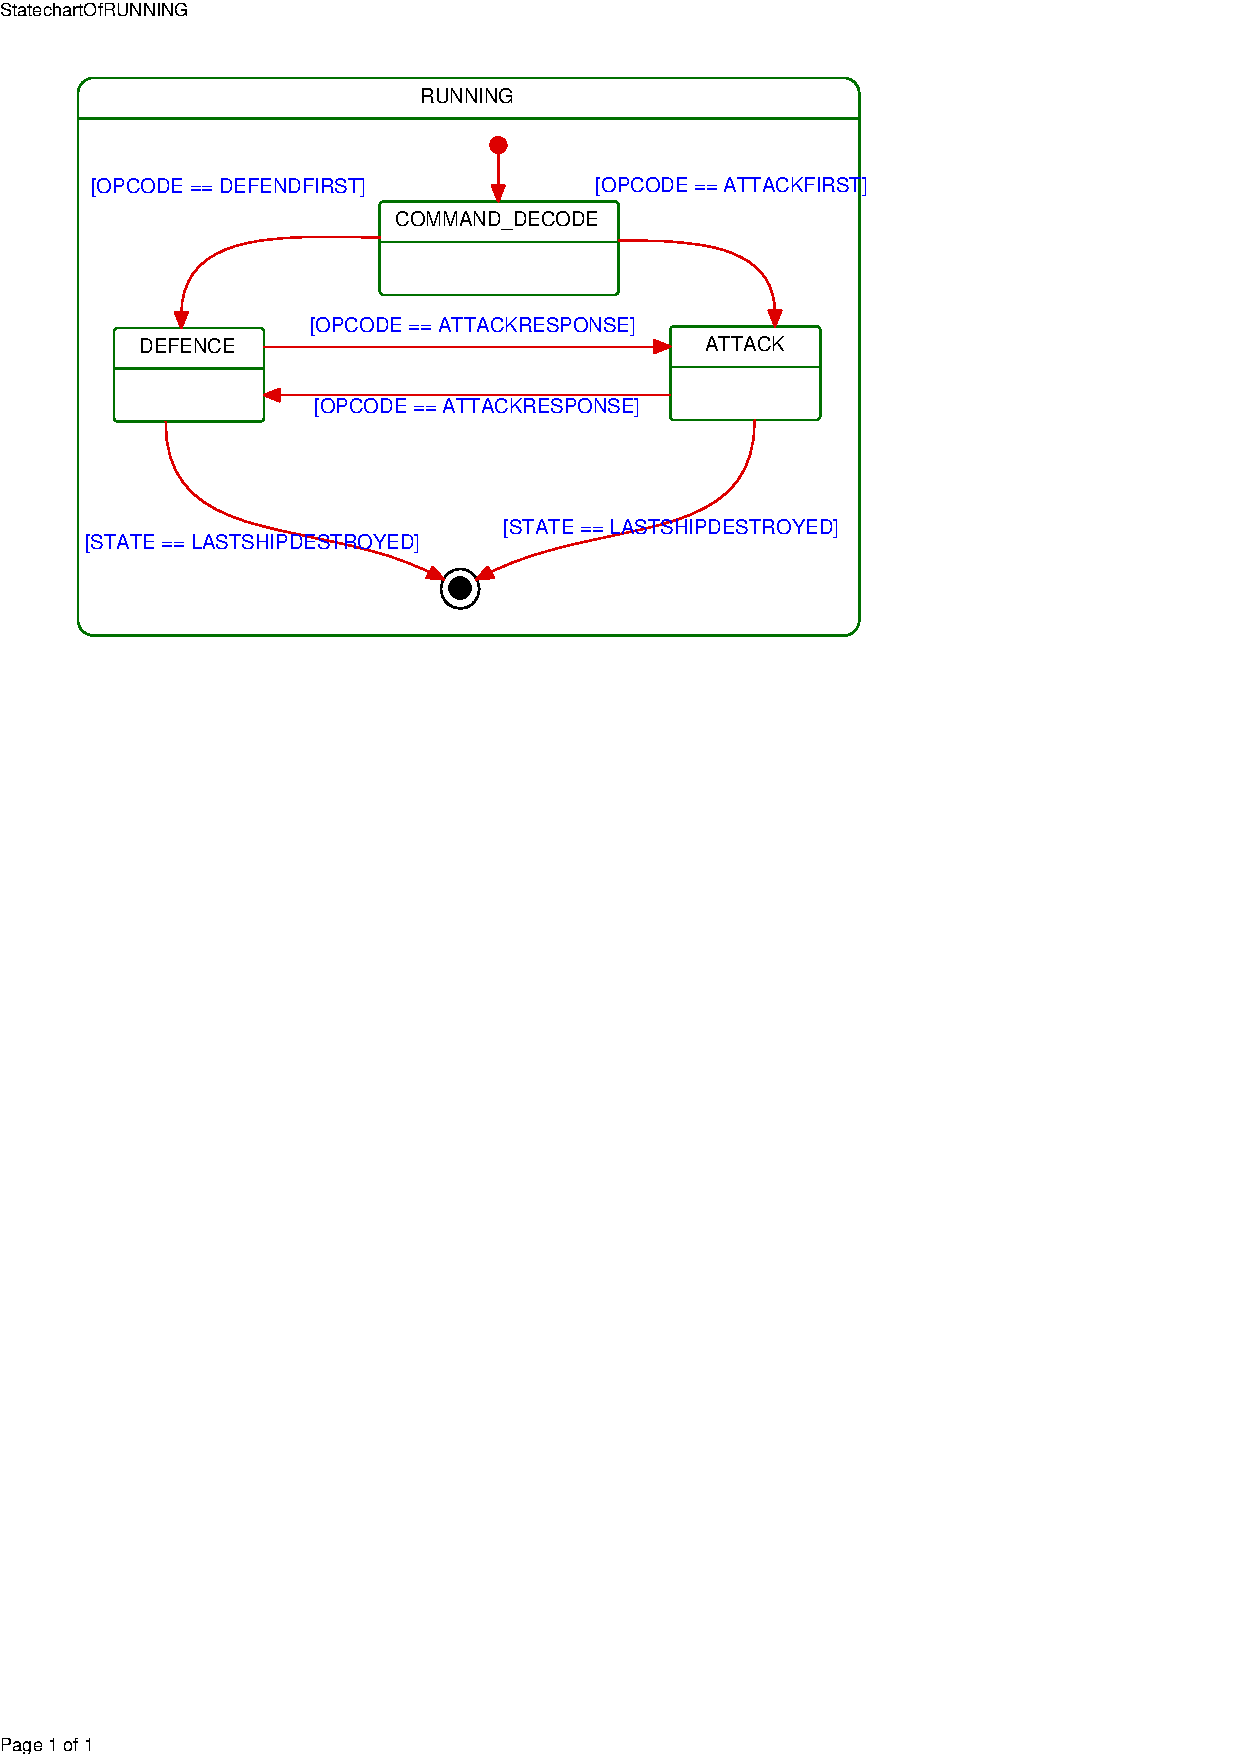
\includegraphics[trim=10mm 185mm 60mm 10mm,clip,width=0.5\textwidth]{images/SubSMRUNNING.pdf}
  \caption{Interne Zustandsübergänge während des laufenden Spiels}
  \label{fig:SubClientstates}
\end{figure}

Die vorgesehene Kommunikationsabfolge wird ebenfalls in Abbildung \ref{fig:Kommunikationssequenz} in Form eines Sequenzdiagramms dargestellt.
Das Diagramm stellt einen beispielhaften Spielablauf mit einem Prolog-Client und einem Java-Client dar. 
Der Client, der sich zuerst mit dem Server verbindet, beginnt per Konvention im Verteidungsmodus und der zweite verbundene Client startet im Angriffsmodus.
Erst wenn sich zwei Teilnehmer am Server verbunden haben, sendet dieser das Startsignal an alle Clients.

Die Spielphase wird durch eine Schleife bestimmt, in der die Teilnehmer von den Angriffs- in den Verteidigungszustand wechseln und umgekehrt.
Die dabei übertragenen Nachrichten werden stets an den Server übertragen, der diese an den jeweils anderen Client weiterleitet.
Dadurch kommt keine direkte Verbindung beider Spieler zustande.

Das Programmende aus Sicht der Kommunikation wird erreicht, wenn ein Spieler die Nachricht überträgt, dass er über keine Schiffe mehr verfügt.
In diesem Fall werden die Verbindungen getrennt und der Server kann neue Verbindungen von Spielern zum Ausrichten eines neuen Spiels annehmen.

\begin{figure}[H]
  \centering
  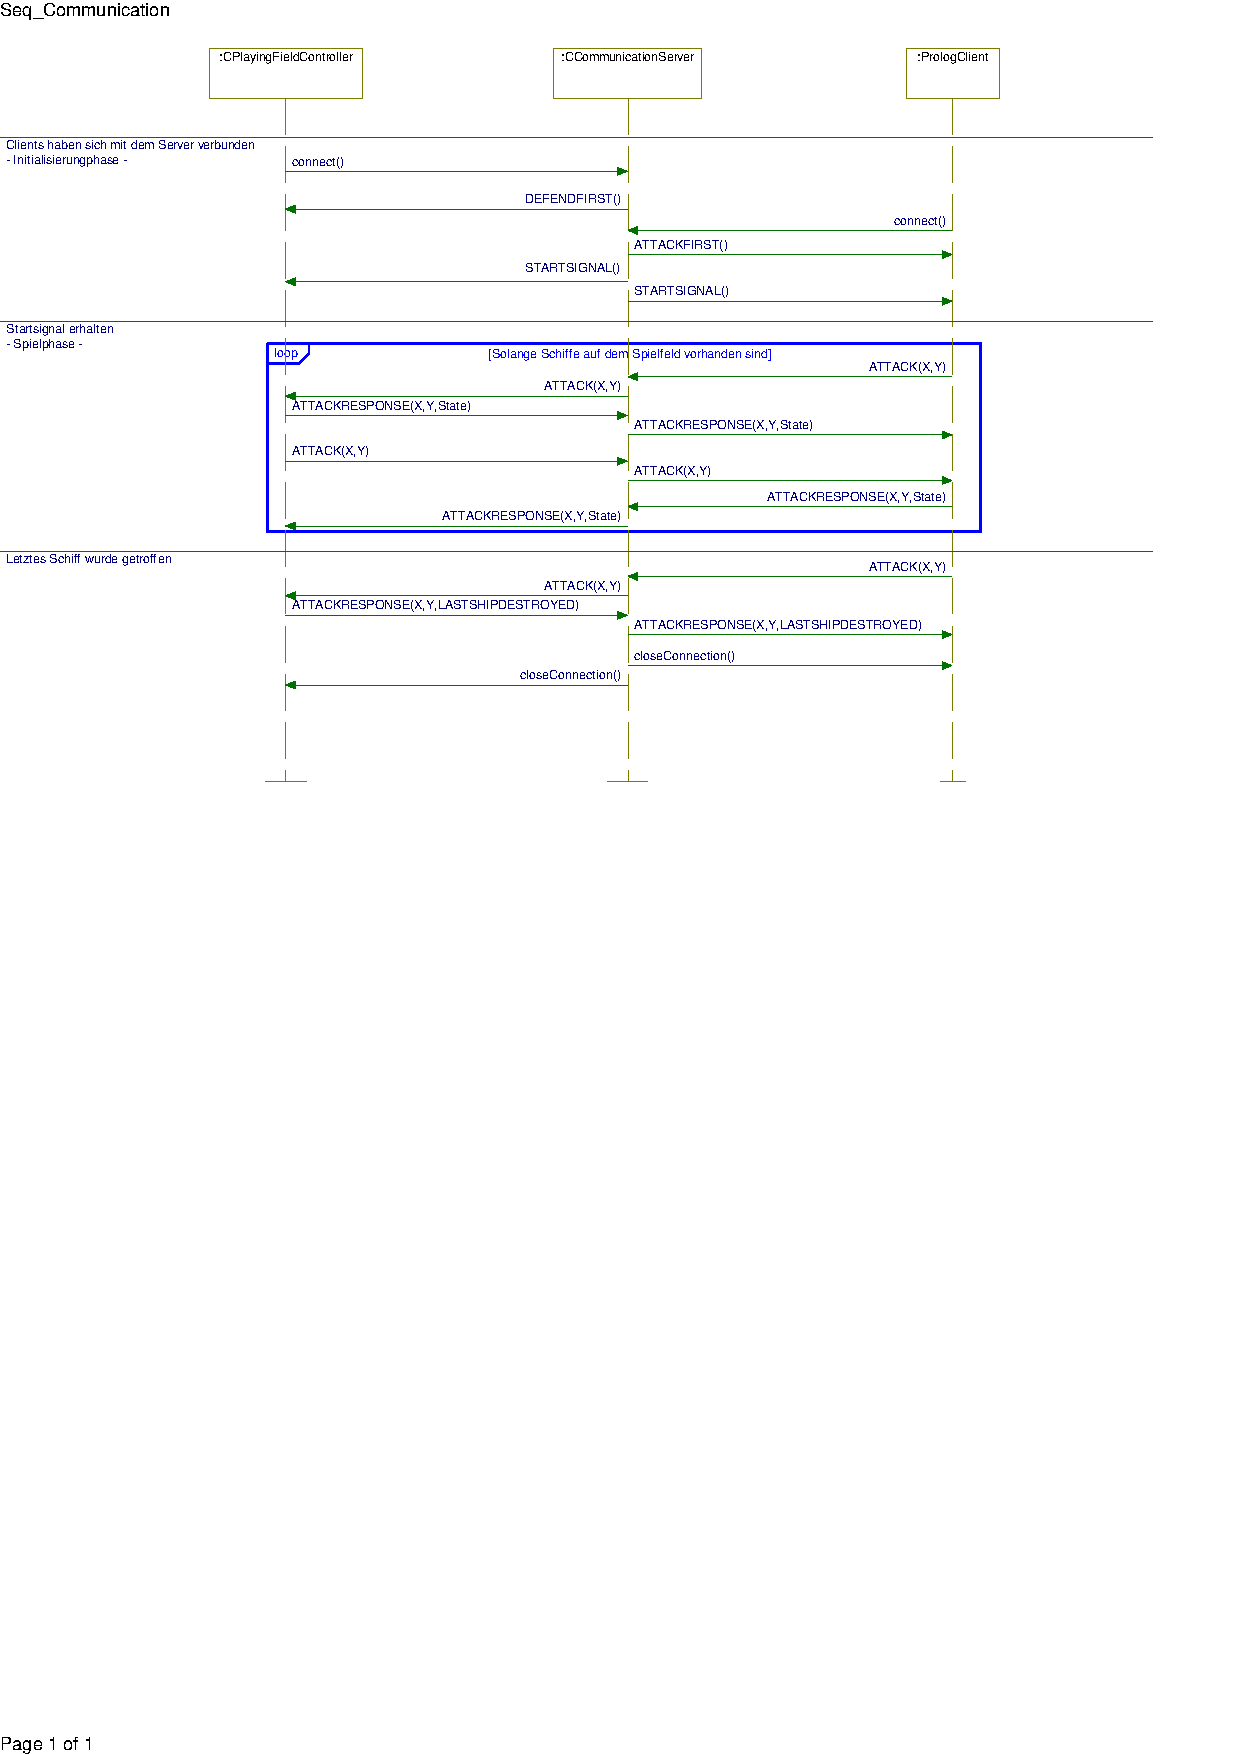
\includegraphics[trim=0mm 160mm 25mm 5mm,clip,width=0.95\textwidth]{images/SeqCommunication.pdf}
  \caption{Sequenzdiagramm der Kommunikation}
  \label{fig:Kommunikationssequenz}
\end{figure}


		\subsection{Spielserver}
\label{sec:Spielserver}

		\subsection{Client - Java}
\label{sec:Javaclient}

Der hier beschriebene Java-Client ist ein möglicher Teilnehmer, der sich mit den Kommunikationsserver verbinden und ein Spiel austragen kann.
Sein Design orientiert sich am Model-View-Controller (MVC) Prinzip, wobei das Spielbrettmodell auf Grund seines geringen Umfangs im Controller eingebettet wurde.

Eine Übersicht des Entwurfs wird in Abbildung \ref{fig:Javaclientklassendiagramm} dargestellt.
Die beiden Klassen \texttt{CBattleShipGUI} und \texttt{CPlayingFieldPanel} bilden den \emph{View} Bestandteil des MVC Prinzips ab.

\begin{figure}[H]
  \centering
  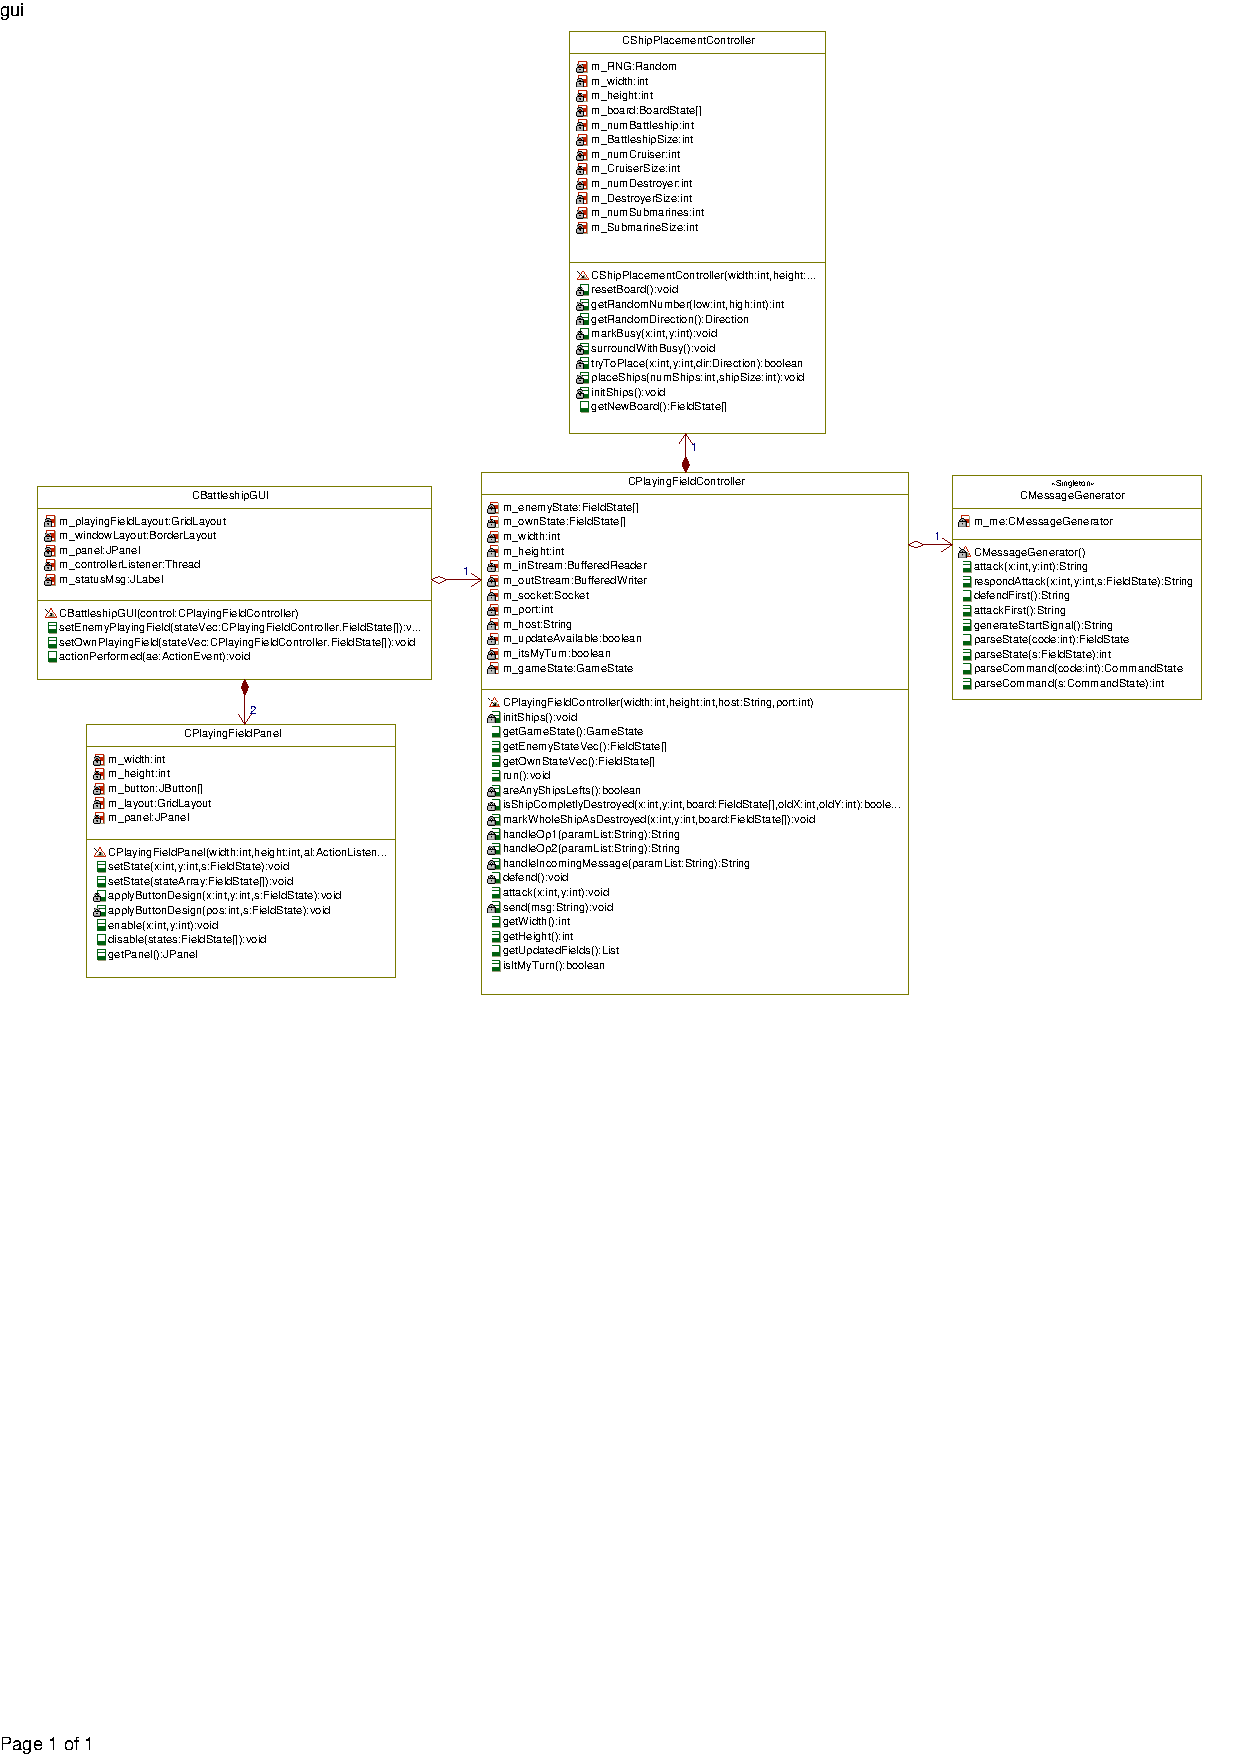
\includegraphics[trim=5mm 82mm 0mm 4mm,clip,width=1.0\textwidth]{images/CJavaClient.pdf}
  \caption{Klassendiagramm des Java Clients}
  \label{fig:Javaclientklassendiagramm}
\end{figure}

%\todoin{Vic - Ich befürchte, dass das Klassendiagramm kaum lesbar ist, macht es dann sinn das reinzunehmen? oder siehst du ne möglichkeit das größer zu machen?}

\subsubsection{View}

Das eigene, sowie das gegnerische Spielfeld werden durch jeweils eine Instanz der Klasse \texttt{CPlayingFieldPanel} visualisiert, wie es in Abbildung \ref{fig:Spielfeldpanel} zu sehen ist.
Dieses besteht primär aus einem gitterförmigen Spielfeld, dessen Spielfeldzustände durch Farben codiert sind.
Das hier gezeigte Spielfeld stellt das eigene Wissen des gegnerischen Spielfelds dar.
Die grauen Felder symbolisieren noch unbekanntes Terrain.
Blau bedeutet, dass bei einem vorangegangenen Angriff ein Feld mit Wasser getroffen wurde.
Rot symbolisiert ein getroffenes, jedoch noch nicht versenktes Schiff.
Versenkte Schiffsfelder sind dunkelgrau gehalten.

\begin{figure}[H]
  \centering
  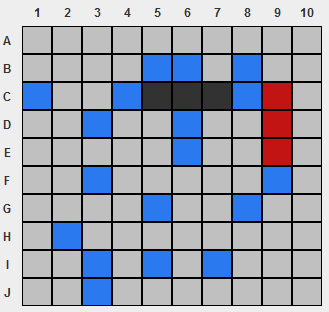
\includegraphics[width=0.5\textwidth]{images/JavaPlayingFieldPanel.png}
  \caption{Gegnerisches Spielfeld mit einem zerstörten (dunkelgrau) und einem beschädigten Schiff (rot)}
  \label{fig:Spielfeldpanel}
\end{figure}

Die visuelle Codierung des eigenen Spielfeldes wird analog zum gegnerischen Feld vorgenommen.
Hier sind standardmäßig alle Felder aufgedeckt und wie in Abbildung \ref{fig:EigenesSpielfeldpanel} zu sehen ist, hellblau eingefärbt.
Die eigenen Schiffe sind ebenfalls sichtbar und mit hellgrauer Farbe hervorgehoben.
Angriffe des Gegners, die das Wasser getroffen haben, sind dunkelblau dargestellt.
Analog zum gegnerischen Spielfeld sind Treffer rot und versenkte Schiffe dunkelgrau eingefärbt.

\begin{figure}[H]
  \centering
  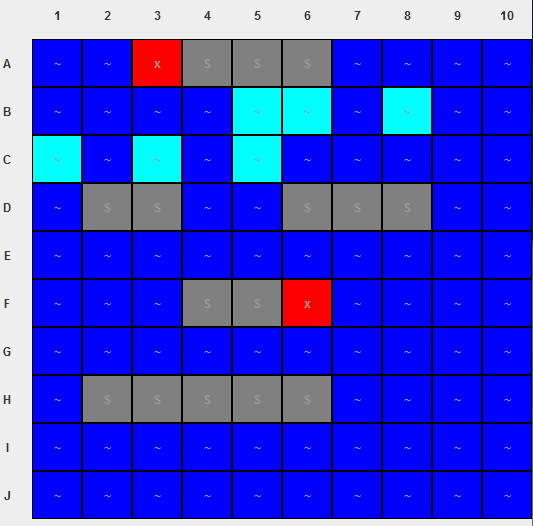
\includegraphics[width=0.5\textwidth]{images/JavaOwnPlayingFieldPanel.png}
  \caption{Eigenes Spielfeld mit versenkten Schiffen (dunkelgrau), einem beschädigten Schiff (rot) und misglückten Angriffen des Gegners (dunkelblau)}
  \label{fig:EigenesSpielfeldpanel}
\end{figure}

Die GUI-Oberfläche besteht primär aus zwei Instanzen der Klasse \texttt{CPlayingFieldPanel}, die jeweils das eigene und gegnerische Spielfeld abbilden.
Wie in Abbildung \ref{fig:GUI} zu erkennen ist, befindet sich über jedem Spielfeld eine Überschrift, die die Zugehörigkeit signalisiert.
Des Weiteren befindet sich in der unteren linken Ecke ein Statusfeld, das angibt, wer den nächsten Spielzug auszuführen hat bzw. ob man das Spiel verloren bzw. gewonnen hat.
Sollte der Gegner am Zug sein, so wird gleichzeitig das gesamte Spielfeld deaktiviert, sodass keine Buttonaktionen ausgeführt werden können.

\begin{figure}[H]
  \centering
  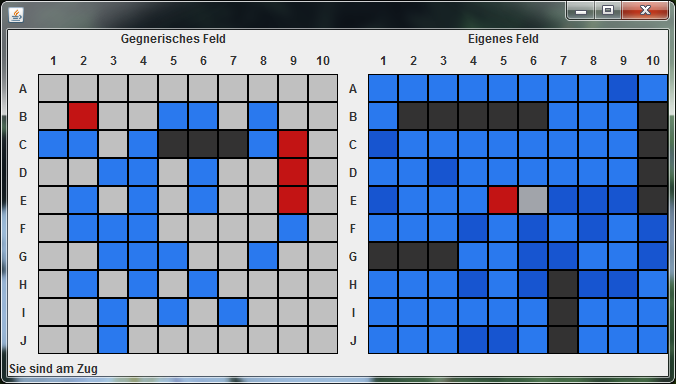
\includegraphics[width=0.9\textwidth]{images/JavaClientGUI.png}
  \caption{Gesamte Benutzeroberfläche}
  \label{fig:GUI}
\end{figure}

\subsubsection{Controller / Model}

Die Klasse \texttt{CPlayingFieldController} ist das zentrale Element der Spielsteuerung und wertet die eingehenden Nachrichten und Signale aus.
Des Weiteren beinhaltet diese Klasse auch die Model-Komponente in Form zweier Arrays, die die Spielfelder repräsentieren.
Der Abruf dieser Daten orientiert sich am Observer Entwurfsmuster.
Jede Änderung an diesen Arrays wird mittels der javaeigenen Methode \texttt{notifyAllObservers()} den Beobachtern mitgeteilt.

Der Controller-Anteil wird durch die Erzeugung eines Threads realisiert, der eingehende Netzwerknachrichten annimmt und auswertet.
Zur Generierung ausgehender Nachrichten, die einen Angriff signalisieren, dient die Methode \texttt{attack(int x, int y)}. Sie wird durch die Interaktion mit der GUI aufgerufen.
Sowohl der Thread, als auch die GUI-Interaktion blockieren sich auf Basis von Monitoren gegenseitig, die mit dem Schlüsselwort \texttt{synchronized} signalisiert werden.
Mittels dieser Technik wird verhindert, dass die beiden Zustände \emph{ATTACK} und \emph{DEFENCE} unsachgemäß eingenommen werden.

Eingehende Angriffe werden durch den Vergleich mit dem eigenen Spielfeld behandelt und das Ergebnis per Nachricht bekannt gegeben.
Gleichzeitig wird der Status des eigenen Spielfeldes an der entsprechenden Stelle aktualisiert.
Im Fall von Wasser wird an dieser Position der Status \textit{Verfehlt} gesetzt.
Bei einem Schiff wird der Status auf \textit{Getroffen} geändert.
Gleichzeitig wird eine Routine gestartet, die überprüft, ob das das ganze Schiff versenkt wurde.
Ist dem so, so wird wiederum eine Routine gestartet, die überprüft, ob alle Schiffe versenkt wurden.
Die entsprechenden Ergebnisse werden per Netzwerkantwort übermittelt.
Sind keine eigenen Schiffe mehr vorhanden, oder ging die Nachricht ein, dass der Gegner über keine Schiffe mehr verfügt, so wird der Spielstatus auf verloren, bzw. gewonnen gesetzt.

Die Generierung der prologkompatiblen Nachrichten wird in der Klasse \texttt{CMes\-sage\-Ge\-ne\-ra\-tor} vorgenommen.
Diese bietet passende Methoden für jede Aktion und Reaktion und liefert den zu übertragenen Text.
Die Klasse ist ebenfalls für die Dekodierung der Opcodes und Ergebnisse in interne Enumerationen zuständig.

In der Initialisierungphase ruft der Controller die Klasse \texttt{CShip\-Place\-ment\-Con\-trol\-ler} auf.
Diese Klasse ist für die regelkonforme Platzierung der Schiffe auf dem Spielbrett zuständig.
Der Vorgang zum Platzieren eines Schiffes ist dabei von seinem Typ und somit seiner Größe unabhängig und kann wie folgt beschrieben werden:
\begin{enumerate}
	\item Generiere zufällig die $x/y$ Position, sowie die Orientierung, in der das Schiff platziert werden soll.
	\item Prüfe ob diese Position belegt ist, oder ob sich in der direkten 4er Nachbarschaft ein Schiff befindet. 
	Es gilt ebenfalls die Spielfeldgrenzen zu berücksichtigen.
	\item Wiederhole den vorherigen Schritt rekursiv an der nächsten Position in angegebener Orientierung. 
	Die Schiffsgröße wird mit jedem Rekursionsschritt um 1 verringert, sodass aus dieser Angabe die Abbruchbedingung erzeugt werden kann.
	\item Wurde in keinem Feld rekursiv eine Behinderung festgestellt, werden die Felder mit der Schiffskennung versehen.
\end{enumerate}
Diese vier Verarbeitungsschritte werden für jedes zu platzierende Schiff aufgerufen.
Jedoch ist nicht gewährleistet, dass eine zufällig generierte Position auch frei ist.
Deshalb steht pro Schiffstyp ein maximales Kontingent an Versuchen zur Verfügung, das sich nach jedem erfolgreich platzierten Schiff wieder füllt.
Sollte das Kontingent für einen Schiffstypen aufgebraucht worden sein, so wird das Gesamtkontingent für das gesamte Spielbrett reduziert und das gesamte Spielbrett wird zurückgesetzt.
Sollte auch dieses Kontingent aufgebraucht worden sein, wird eine Fehlermeldung per Exception ausgegeben.
		\subsection{Client - Prolog} \label{sec:Prologclient}
	Die Aufgaben des Prolog-Clients sind in verschiedene Module unterteilt, um die verschiedenen Teile austauschbar zu halten. 
	Abbildung \ref{fig:prologmodule} zeigt das Zusammenspiel der Module. Dabei stellt ein Pfeil die Verwendung eines Prädikates aus
	dem jeweiligen Modul dar. Die im Diagramm dargestellten Pfeile stellen somit die Schnittstellen zwischen den Modulen dar.
	
	\begin{figure}[H] % (fold)
		\centering
		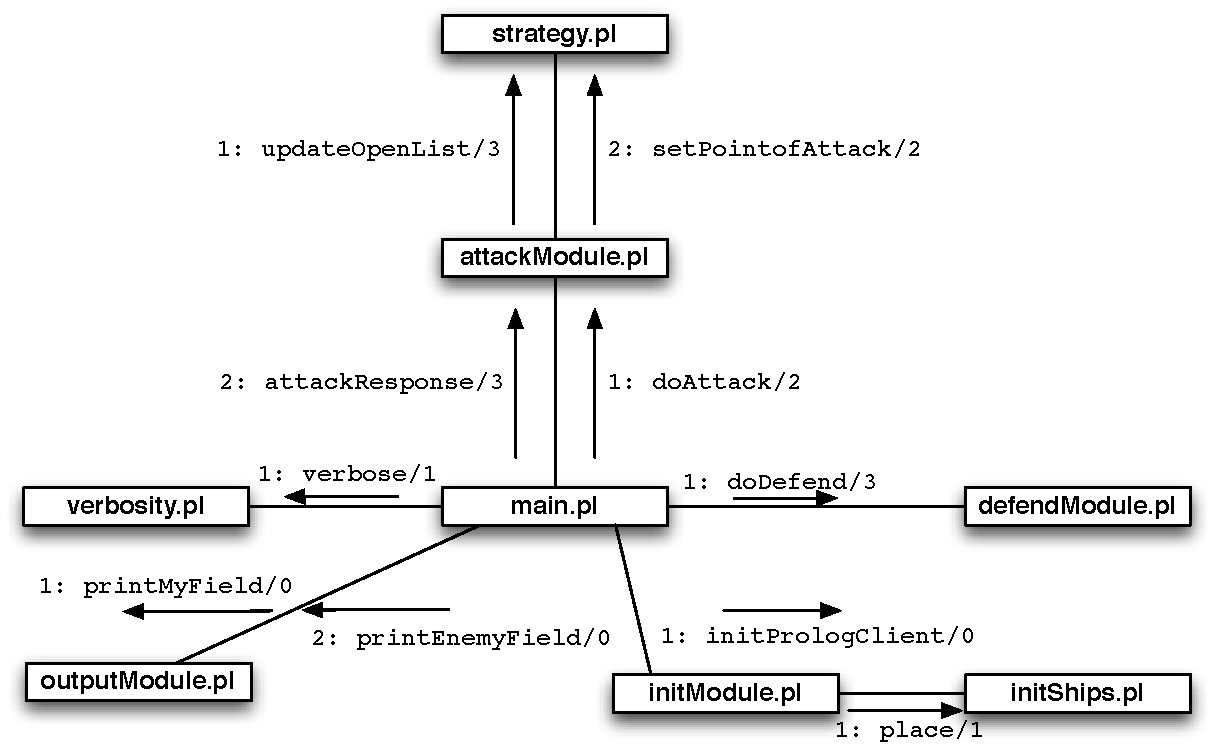
\includegraphics[width=0.9\textwidth]{images/ModuleCommunication.pdf}
		\caption{UML Kommunikationsdiagramm zur Kommunikation zwischen den Modulen des Prolog-Clients}
		\label{fig:prologmodule}
	\end{figure}
	% figure fig:prologmodule (end)

	Des Weiteren arbeiten einige der Module gemeinsam auf \textit{globalen} Spielvariablen, die mit Hilfe von dynamischen Prädikaten
	gespeichert werden. Tabelle \ref{tbl:globalevariablen} zeigt diese Variablen, ihren Zweck sowie ihre Verwendung auf.
	
	%\begin{table}[H]
	%	\centering
		\begin{longtable}{|l|p{6cm}|p{5cm}|}
			\hline
			Prädikat & Zweck & Verwendet von \\ 
			\hline 
			\hline \endhead
			\texttt{myField/1} & Speichert Zustand des eigenen Spielfeldes & Initialisierungsmodul, Verteidigungsmodul, Ausgabemodul \\
			\hline
			\texttt{enemyField/1} & Speichert Zustand des gegnerischen Spielfeldes & Initialisierungsmodul, Strategiemodul, Angriffsmodul, Ausgabemodul \\
			\hline
			\texttt{openList/1} & Speichert Liste der bevorzugt anzugreifenden, gegnerischen Felder & Initialisierungsmodul, Strategiemodul, Ausgabemodul \\
			\hline
			\texttt{numberOfGames/1} & Speichert Verbleibende Anzahl von Spieldurchgängen (für aufeinander folgende Durchgänge) & Hauptmodul \\
			\hline
			\texttt{numberOfWins/1} & Speichert die Anzahl der bisher gewonnenen Spiele (für aufeinander folgende Durchgänge) & Hauptmodul \\
			\hline
			\texttt{numberOfLosses/1} & Speichert die Anzahl der bisher verlorenen Spiele (für aufeinander folgende Durchgänge) & Hauptmodul \\
			\hline
			\texttt{currentStream/1} & Speichert den aktuell gesetzten Ausgabestrom (Konsole, Datei, keiner) & Hauptmodul, Ausgabemodul \\
			\hline
%		\end{tabular}
		\caption{Prädikate für globale Spielvariablen}
		\label{tbl:globalevariablen}
	\end{longtable}
	
	Im Folgenden werden die Aufgaben und die Funktionsweise der verschiedenen Module erläutert.

\subsubsection{Hauptmodul} \label{sec:hauptmodul}
	Das Hauptmodul \texttt{main.pl} wird beim Starten des Clients aufgerufen. Der Client bietet die Möglichkeit eine konfigurierbare Anzahl
	von Runden zu spielen. Dies wird vorallem bei Spielen verwendet, in denen zwei \textit{Computergegner} gegen einander antreten. 
	Beim Start des Clients werden deshalb zunächst die Anzahl der Spiele, Siege sowie Niederlagen initialisiert und in den Prädikaten
	\texttt{numberOfGames/1}, \texttt{numberOfWins/1} sowie \texttt{numberOfLooses/1} gespeichert. Außerdem wird der gewünschte Ausgabestream
	im Prädikat \texttt{verbose/1} hinterlegt.
	
	Für jedes neue Spiel initialisiert das Modul zunächst die Verbindung zum
	Spielserver. Anschließend werden Spielvorbereitungen über das Prädikat \texttt{initPrologClient/0} aus dem 
	Initialisierungsmodul getroffen (siehe Abschnitt \ref{sec:initModule}).
	
	Je nachdem ob der Client im Angriffs- oder Verteidigungsmodus startet, werden die Prädikate \texttt{attackFirst/0} oder
	\texttt{defendFirst/0} aufgerufen. Nach Empfang des Startsignals beginnt der Client dann mit einem Angriff oder Verteidigung.
	
	Ein Angriff verwendet die Prädikate \texttt{doAttack/2} und \texttt{attackResponse/3} des Angriffsmoduls (siehe Abschnitt
	\ref{sec:attackModule}).
	Das Prädikat \texttt{doAttack/2} liefert den Punkt auf dem gegnerischen Spielfeld der angegriffen werden soll.
	Die so erhaltenen X-Y-Koordinaten gibt das Hauptmodul an den Server weiter und wartet anschließend auf eine Antwort des 
	Gegners (über den Server). 
	Nach Erhalt dieser Antwort verwendet das Hauptmodul das Prädikat \texttt{attackResponse/3}, um die Antwort zu verarbeiten.
	Mit Abschluss der Verarbeitung ist der Angriff beendet.
	
	Die Verteidigung verwendet das Prädikat \texttt{doDefend/3} des Verteidigungsmoduls (siehe Abschnitt \ref{sec:defendModule}).
	Zu Beginn der Verteidigung wartet das Hauptmodul zunächst auf den Angriff des Gegners. Die so erhaltenen Koordinaten
	werden an das Prädikat \texttt{doDefend/3} übergeben. Als Resultat liefert dieses Prädikat die entsprechende Antwort für den
	Gegner. Das Hauptmodul sendet die Antwort gemäß dem Kommunikationsprotokoll an den Server. Damit ist die Verteidigung 
	beendet.
	
	Nach jedem Angriff überprüft der Client, ob er das Spiel gewonnen hat. Gleichermaßen überprüft er nach jeder Verteidigung, 
	ob er das Spiel verloren hat. Tritt einer der beiden Fälle in Kraft, so beendet der Client das Spiel. 
	Anschließend überprüft der Client ob weitere Runden ausstehen. Ist dies der Fall, so wird ein neues Spiel initialisiert.
	Andernfalls beendet sich der Client mit einer Ausgabe über den Spielverlauf:
	\textit{End of game. KI won \texttt{n} times and lost \texttt{m} times.}.

\subsubsection{Initialisierungsmodul} \label{sec:initModule}
	Die Aufgaben des Initialisierungsmoduls \texttt{initModule.pl} sind das Initialisieren der Spielfelder, darunter auch
	das Platzieren der eigenen Schiffe, sowie das Initialisieren der Openlist für primär anzugreifende Felder (siehe Abschnitt \ref{sec:strategy}).
	
	Zur Initialisierung der Spielfelder verwendet das Modul die Prädikate \texttt{initMyField/0} und \texttt{initEnemyField/0}.
	Die Spielfelder werden global in den dynamischen Prädikaten \texttt{myField/1} und \texttt{enemyField/1}
	gespeichert, um einen einfachen Zugriff von jedem Modul zu ermöglichen. 
	
	Zur Platzierung der eigenen Schiffe verwendet das Initialisierungsmodul das Prädikat \texttt{place/1} aus dem Modul zur 
	Schiffspositionierung (\texttt{initShips.pl}, siehe Abschnitt \ref{sec:initships}).
	Die von \texttt{place/1} gelieferte Liste beinhaltet (unter anderem) die Koordinaten der Schiffe, welche durch das Prädikat 
	\texttt{fillWithShips/3} im eigenen Spielfeld \texttt{myField/1} als belegt gekennzeichnet werden. Hierfür wird 
	die von \texttt{place/1} bezogene Liste rekursiv abgearbeitet und die enthaltenen X-Y-Koordinaten in \texttt{MyField/1} mit dem 
	Status 6 belegt. Dieser Status sagt im Prolog-Client aus, dass sich auf der Koordinate ein Teil eines Schiffes befindet.
	
	Die Listenelemente enhalten neben den Koordinaten noch eine Nummer zur Identifizierung des Schiffes, sowie die "'Teilenummer"' 
	die angibt um den wievielten Teil eines Schiffes es sich handelt. Getrennt sind diese Komponenten durch einen Schrägstrich. Somit 
	stellt sich ein Listenelement wie folgt dar: \texttt{Schiffs-ID}/ \texttt{Teilnummer}/ \texttt{X-Koordinate}/ \texttt{Y-Koordinate}.
	Die X- und Y-Koordinate müssen zur korrekten Verwendungen jeweils noch einmal dekrementiert werden, weil im Modul \texttt{initShips.pl} von 
	einem Koordinatensystem mit den Wertebereichen $1\le X/Y\le 10$ ausgegangen wird, während \texttt{myField/1} vom Wertebereich $0\le X/Y\le 9$ ausgeht.
	
	Die folgende Abbildung \ref{fig:fillwithShips3} bildet diesen Ablauf schematisch, als UML-Diagramm, ab. Die abgebildete Schleife 
	wird in Prolog durch Rekursion realisiert.
	\begin{figure}[H] % (fold)
		\centering
		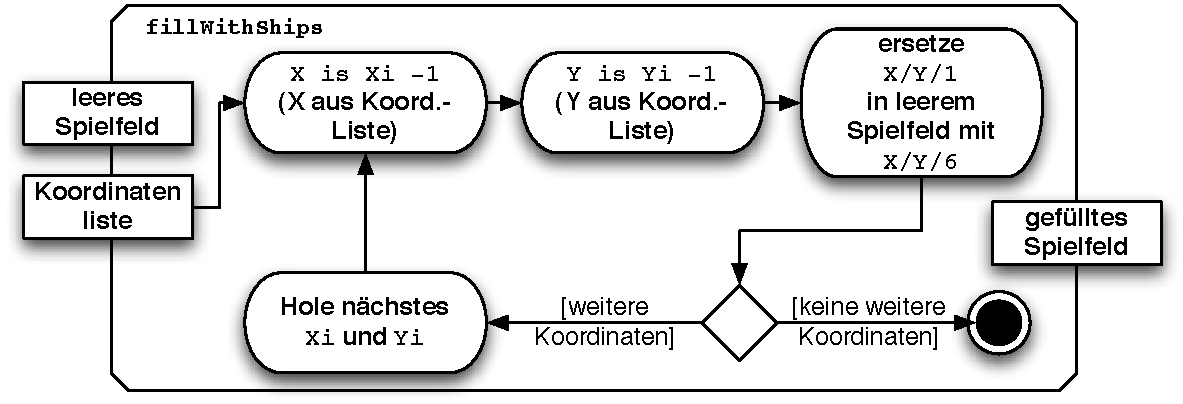
\includegraphics[width=.9\textwidth]{images/fillWithShips.pdf}
		\caption{UML Aktivitätsdiagramm des Prädikats \texttt{fillWithships/3}. \emph{Quelle: Eigene Darstellung.}}
		\label{fig:fillwithShips3}
	\end{figure}
	% figure fig:fillwithShips3 (end)

\subsubsection{Modul zur Plazierung von Schiffen} \label{sec:initships}	
	Die Aufgabe des Positionierungsmoduls \texttt{initShips.pl} ist es, die Schiffe der künstlichen Intelligenz auf dem Spielfeld zu platzieren.
	Hierfür werden in diesem Modul die Regeln zur legalen Positionierung der Schiffe (siehe Abschnitt \ref{sec:Spielregeln}) implementiert. Neben den Regeln 
	zur Platzierung definiert \texttt{initShips.pl} auch die Anzahl und Länge der im Spiel genutzten Schiffe. Des weiteren wurden Prädikate implementiert, 
	welche die Regeln auf die Menge der Schiffe Anwenden um so mögliche Positionierungen dieser auf dem Spielfeld zu erzeugen.
	
	Das Prädikat \texttt{place/1} stößt die Erzeugung einer zufälligen Aufstellung aller Schiffe auf dem Spielfeld an und gibt diese als Liste der Form 
	\texttt{Schiffs-ID}/ \texttt{Teilnummer}/ \texttt{X-Koordinate}/ \texttt{Y-Koordinate} an.
	
	Um sicherzustellen das nur legale Positionierungen verwendet werden, wurden die Spielregeln (siehe Abschnitt \ref{sec:Spielregeln}) wie folgt implementiert:
	\begin{itemize}
		\item Schiffe dürfen Horizontal oder Vertikal auf dem Spielfeld platziert werden.\newline
		\lstset{language=Prolog,caption=Implementierung der Platzierungsregel in Prolog,label=code:PrologRules1,	   
		inputencoding=latin1,extendedchars=true,basicstyle=\footnotesize,numbers=left,numberstyle=\footnotesize}
		\lstinputlisting[firstline=29, lastline=46]{includes/initShips.pl}
		\item Verschiedene Schiffe dürfen einander nicht berühren, aber diagonal versetzt stehen.
		\lstset{language=Prolog,caption=Implementierung der Platzierungsregel in Prolog,label=code:PrologRules2,	   
		inputencoding=latin1,extendedchars=true,basicstyle=\footnotesize,numbers=left,numberstyle=\footnotesize}
		\lstinputlisting[firstline=47, lastline=68]{includes/initShips.pl}
	\end{itemize}
	Die Anwendung dieser Regeln erfolgt durch die Abfolge rekursiver Prädikate, welche eine Liste von legal Positionierten Schiffen aufbauen. Es wird also 
	erst ein Schiff auf dem Spielfeld Positioniert, dann ein Zweites dazu gesetzt, darauf folgt das dritte Schiff und so weiter, bis alle fünf Schiffe Positioniert 
	sind. Um eine möglichst zufällige und unvorhersehbare Positionierung der Schiffe zu erreichen werden, da wo es möglich ist, Sequenzen von Zufallszahlen anstatt 
	fest kodierter Listen genutzt. Folgendes UML-Diagramm (Abb. \ref{fig:itShips}) stellt den diesen Ablauf schematisch und vereinfacht dar.
	\begin{itemize}
		\item Das \texttt{Template} ist eine Liste, welche die Schiffe und Eigenschaften (die Länge) beschreibt. Für ein fünf Teile langes Schiff, finden sich im 
		Template fünf Elemente der Form \texttt{Schiffs-ID: 1-5}/ \texttt{Teilenummer: 1-5}/ \texttt{X-Koordinate: Variabel}/ \texttt{Y-Koordinate: Variabel}.
		\item Zu Beginn der Positionierung wird die Reihenfolge, in der die Schiffe platziert werden, zufällig Festgelegt. Hierfür wird eine zufällig Sequenz der 
		Zahlen 1 bis 5 erzeugt und in der Liste \texttt{ships} gespeichert.
	\end{itemize}
	\begin{figure}[H] % (fold)
		\centering
		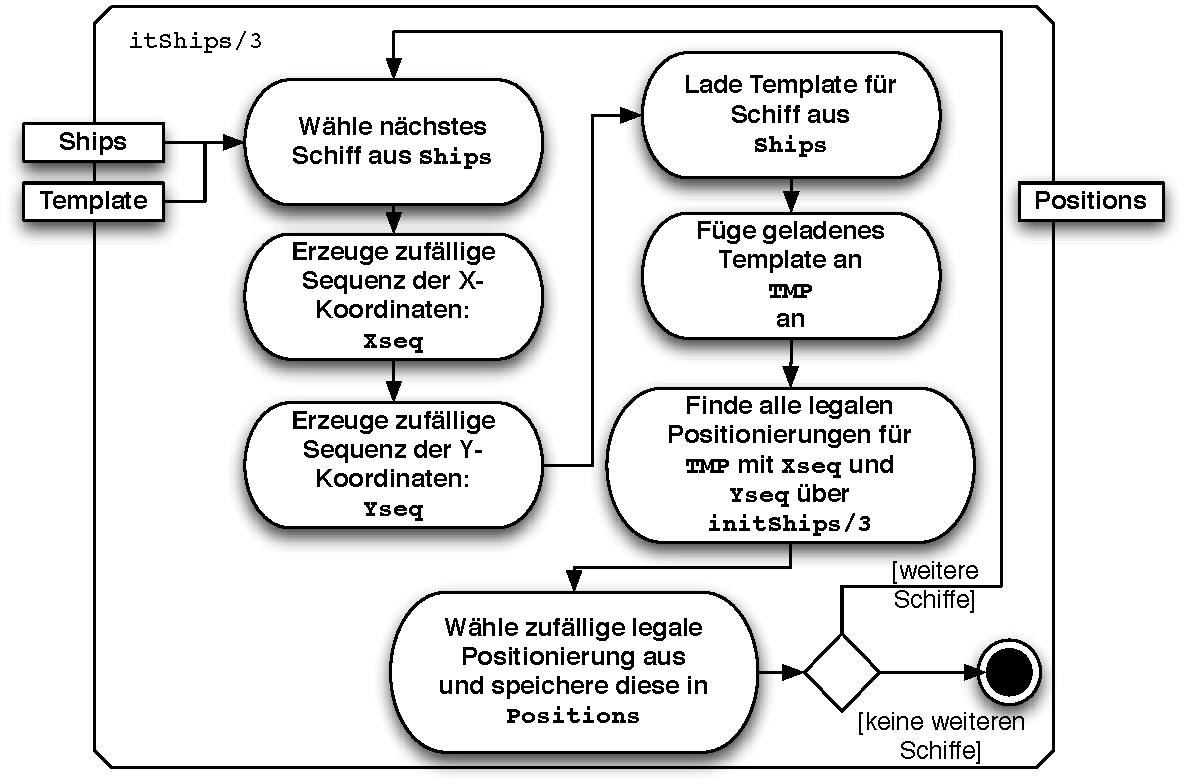
\includegraphics[width=0.9\textwidth]{images/itShips3.pdf}
		\caption{UML-Aktivitätsdiagramm zum Prädikat \texttt{itShips/3}}
		\label{fig:itShips}
	\end{figure}
	% figure fig:initShips (end)
	Auch in \texttt{itShips/3} ist die, in Abbildung \ref{fig:itShips} dargestellte Schleife, als rekursiver Prädikatsaufruf implementiert 
	(vgl. Abschnitt \ref{sec:initModule} und Abbildung \ref{fig:fillwithShips3}).
	
	Das Prädikat \texttt{initShips/3}, welches in Abbildung \ref{fig:itShips} referenziert wird, wendet die in Listing \ref{code:PrologRules1} 
	und \ref{code:PrologRules2} dargestellten 
	Regeln auf die übergebene Liste von Schiffen an. Hierfür werden die übergeben X- und Y-Sequenzen (\texttt{Xseq}, \texttt{Yseq}; die Wertebereiche des Koordinatensystems, 
	welches das Spielfeld abbildet) der Reihe nach abgearbeitet und somit alle legalen Positionierungen für die übergebene Schiffsliste gefunden. Aufgrund der 
	Tatsache, dass immer nur ein Schiff mit Variablen X- und Y-Koordinaten in der übergebenen Liste vorhanden ist (andere, ggf. vorhandene Schiffe, haben bereits 
	in vorherigen durchläufen Koordinaten zugewiesen bekommen), hält sich der Rechenaufwand und die Anzahl der möglichen Positionierungen klein und Prolog kann 
	eine Menge an Lösungen finden und zurück geben.
\subsubsection{Verteidigungsmodul} \label{sec:defendModule}
	Die Aufgabe des Verteidigungsmoduls \texttt{defendModule.pl} ist es einen Angriff des Gegners zu verarbeiten.
	Zum einen muss dabei der Status des eigenen Feldes \texttt{myField/1} aktualisiert 
	und zum anderen die Antwort für den Gegner bestimmt werden.
	
	Hat der Gegner ins Wasser geschossen, so ist keine Änderung des eigenen Feldes notwendig. Trifft der Gegner jedoch ein Schiff,
	so muss ermittelt werden, ob dieser Treffer das Schiff lediglich getroffen oder sogar versenkt hat. Außerdem ändert sich die Antwort
	für den Gegner, wenn das letzte Schiff versenkt wurde.
	
	Ob das letzte Schiff versenkt wurde, erfolgt mit Hilfe einer Abfrage nach verbleibenden Schiffen (Feldstatus 6) im Prädikat \texttt{myField/1}.
	
	Die Überprüfung, ob ein Schiff vollständig versenkt wurde, erfolgt über eine rekursive Überprüfung der 4 benachbarten Felder.
	Dabei erhöht sich die Rekursionstiefe, wenn ein Nachbarfeld ebenfalls als getroffen markiert ist. 
	Da in den Regeln festgelegt ist, dass Schiffe sich nicht berühren dürfen, kann mit diesem Vorgehen festgestellt werden, ob ein Schiff
	vollständig versenkt wurde, oder sich unter den Nachbarn noch ungetroffene Teile befinden.
	
	Schlägt die zuletzt erläuterte Überprüfung fehl, so wurde nur ein Teil eines Schiffes getroffen. Und die entsprechende Antwort wird zurück 
	gegeben.
	
	
\subsubsection{Angriffsmodul} \label{sec:attackModule}
	Die Aufgabe des Angriffsmoduls \texttt{attackModule.pl} ist es, eine Koordinate für den nächsten Angriff zu liefern und außerdem den 
	Rückgabewert des Angriffs zu verarbeiten. 
	Dafür werden die Prädikate \texttt{doAttack/2} und \texttt{attackResponse/3} verwendet. 
	
	Wird das Prädikat \texttt{doAttack} aufgerufen, so nutzt das Angriffsmodul zunächst das Prädikat \texttt{getPointOfAttack/2} des
	Strategiemoduls, um den als nächstes zu attackierenden Punkt zu erhalten. Anschließend überprüft \texttt{doAttack/2} 
	ob die erhaltene Koordinate im Feld des Gegners \texttt{enemyField/1} als unbekannt (Status 0) gilt (Prädikat \texttt{doAttackCheck}. 
	Ist dies nicht der Fall, so wird eine neue Koordinate von \texttt{getPointOfAttack/2} angefordert. 
	Gilt die Koordinate als unbekannt, so wird dieser Punkt als nächster Angriffspunkt zurück gegeben.
	
	Das Prädikat \texttt{attackResponse/3} verarbeitet die Antwort des Gegners auf einen Angriff. Zum einen wird das intern gehaltene, 
	gegnerische Feld aktualisiert (\texttt{updateEnemyField/3}), zum anderen wird die Openlist für weitere Angriffe über 
	das Prädikat \texttt{updateOpenList/3} aus dem Strategiemodul aktualisiert (siehe Abschnitt \ref{sec:strategy}).
	
	Zur Aktualisierung des gegnerischen Spielfeldes \texttt{enemyField/1} wird der vom Gegener erhaltene Status in das entsprechende 
	Feld eingetragen. Eine Ausnahme besteht für die Antwort \textit{Schiff vollständig versenkt}, in diesem Fall wird das ensprechende
	Feld lediglich mit dem Status \textit{Treffer} belegt, um die Handhabung des Spielfeldes zu erleichtern. 

	\subsubsection{Strategiemodul} \label{sec:strategy}

Das Strategiemodul \texttt{strategy.pl} stellt das Prädikat zur Bestimmung des nächsten Angriffspunktes \texttt{getPointOfAttack/2}	zur Verfügung. 
Außerdem füllt dieses Modul die Liste der priorisiert anzugreifenden Punkte über das Prädikat \texttt{updateOpenList/3}. 

Beim Aufruf von \texttt{getPointOfAttack/2} wird das erste Element der Openlist \texttt{openList/2} zurückgegeben.
Befinden sich keine Koordinaten in der Openlist \texttt{openList/1}, so gibt \texttt{getPointOfAttack/2} einen zufälligen Angriffspunkt zurück.

Das Prädikat \texttt{updateOpenList/3} erhält die angegriffene Koordinate und den vom Gegner erhaltenen Rückgabewert. 
Traf der Angriff Wasser oder das letzte Schiff des Gegners, so wird lediglich die angegriffene Position aus der Openlist gelöscht.

Wurde das gerade attackierte Schiff vollständig versenkt, so kann die aktuelle Openlist vollständig geleert werden, da stets nur ein Schiff attackiert wird. 
Außerdem werden die unmittelbar benachbarten Felder des versenkten Schiffes als \textit{Wasser} markiert, denn aufgrund der Spielregeln darf sich auf diesen Feldern kein weiteres Schiff befinden (Prädikat \texttt{surroundWithWater/4}). 

Ist die Antwort des Gegeners \textit{Treffer}, so muss die Openlist aktualisiert werden. 
Dazu werden zunächst alle benachbarten Felder in die Openlist eingetragen, deren Status unbekannt ist (Prädikat \texttt{appendFreeFieldToList/2}). 

Als mögliche Kandidaten der Openlist gehen die Felder der direkten 4er-Nachbarschaft des Treffers ein, wie es in Abbildung \ref{fig:ErstelleOpenlist} zu sehen ist.
Die Reihenfolge wurde auf Westen, Osten, Norden, Süden festgelegt.
\begin{figure}[H]
  \centering
  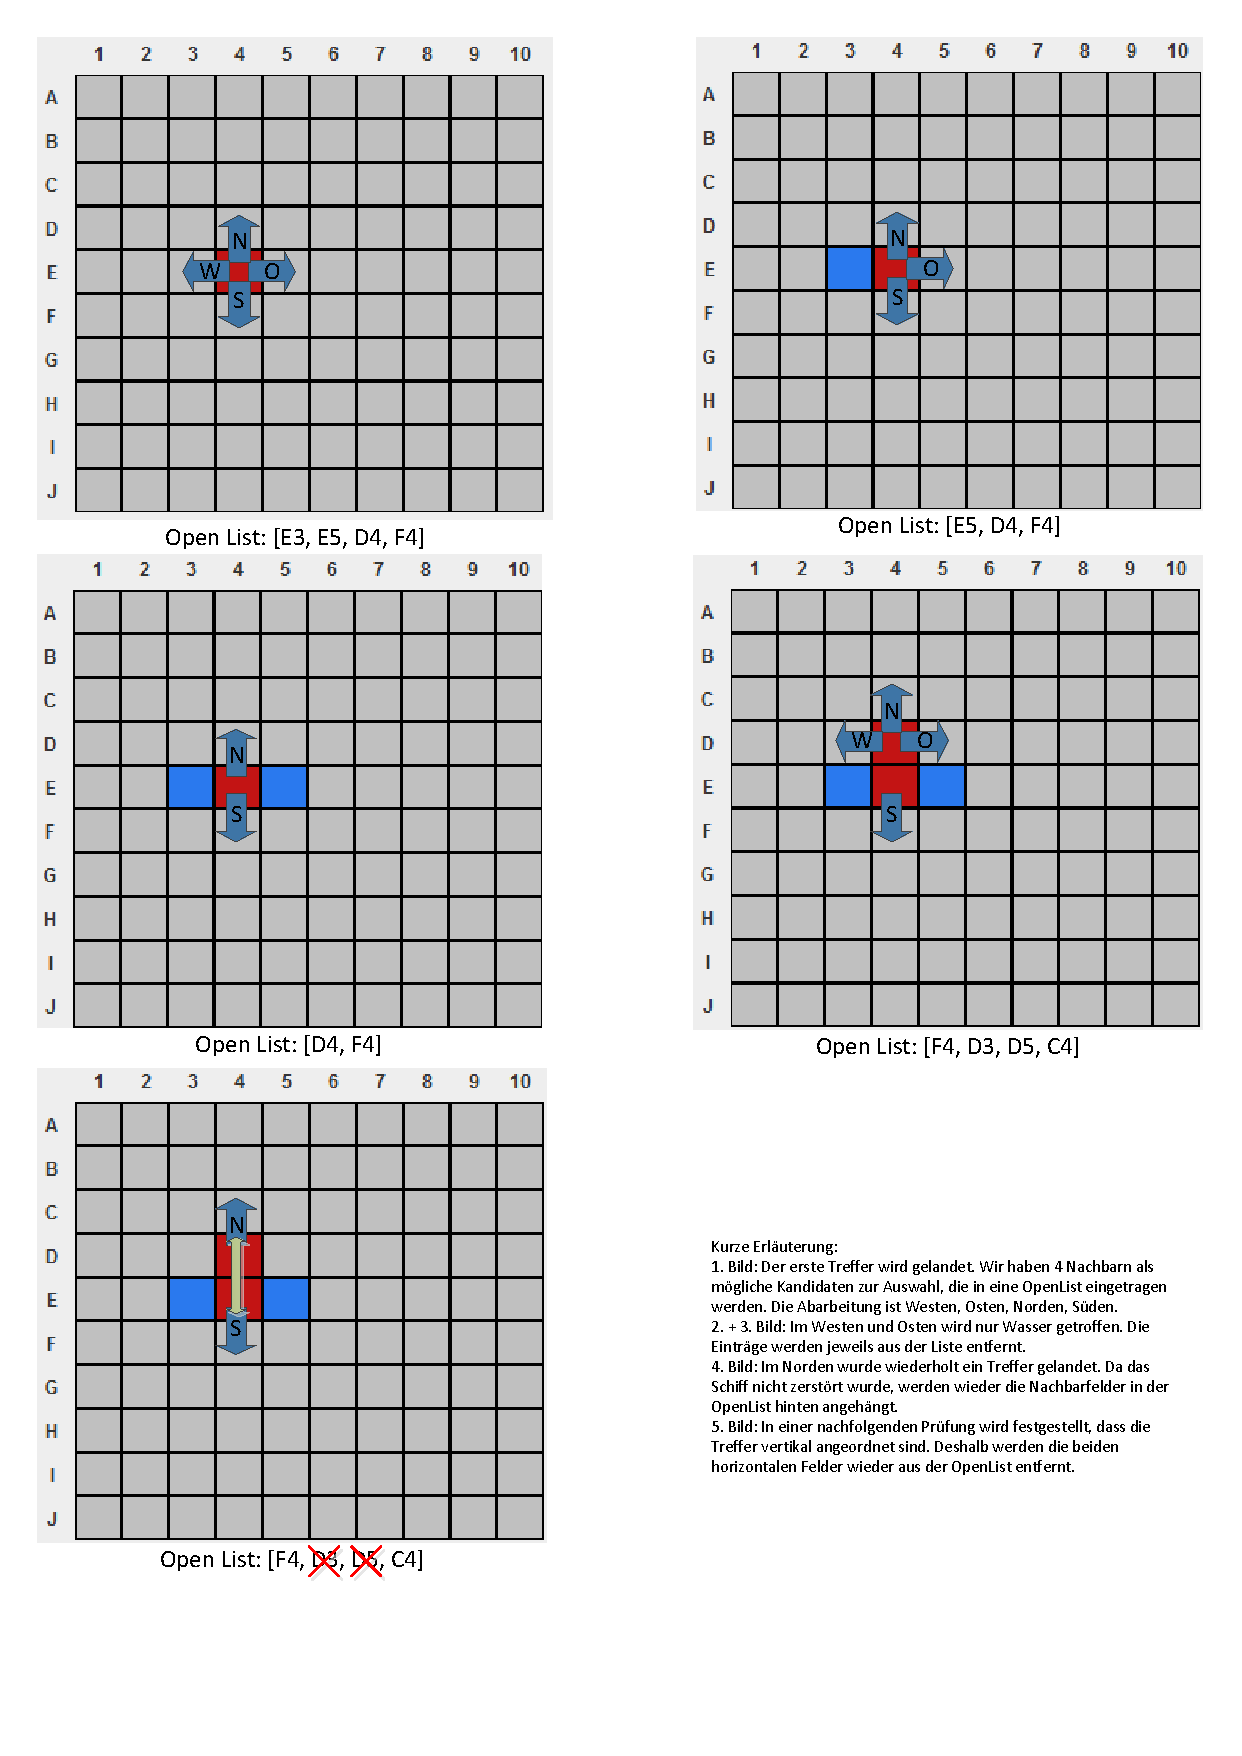
\includegraphics[trim=5mm 204mm 105mm 4mm,clip,width=0.5\textwidth]{images/Strategie_1_FirstHit.pdf}
  \caption{Openlist mit benachbarten Feldern initialisieren}
  \label{fig:ErstelleOpenlist}
\end{figure}

In den nachfolgenden Spielzügen werden diese Felder geprüft.
Sollten diese sich als "'Wasser"' herausstellen, wie es in der Abbildung \ref{fig:Openlist2} angedeutet ist, so werden die entsprechenden Einträge ohne weitere Verarbeitung aus der Openlist gelöscht.
\begin{figure}[H]
  \centering
  \subfigure[Westen (verfehlt)]{
    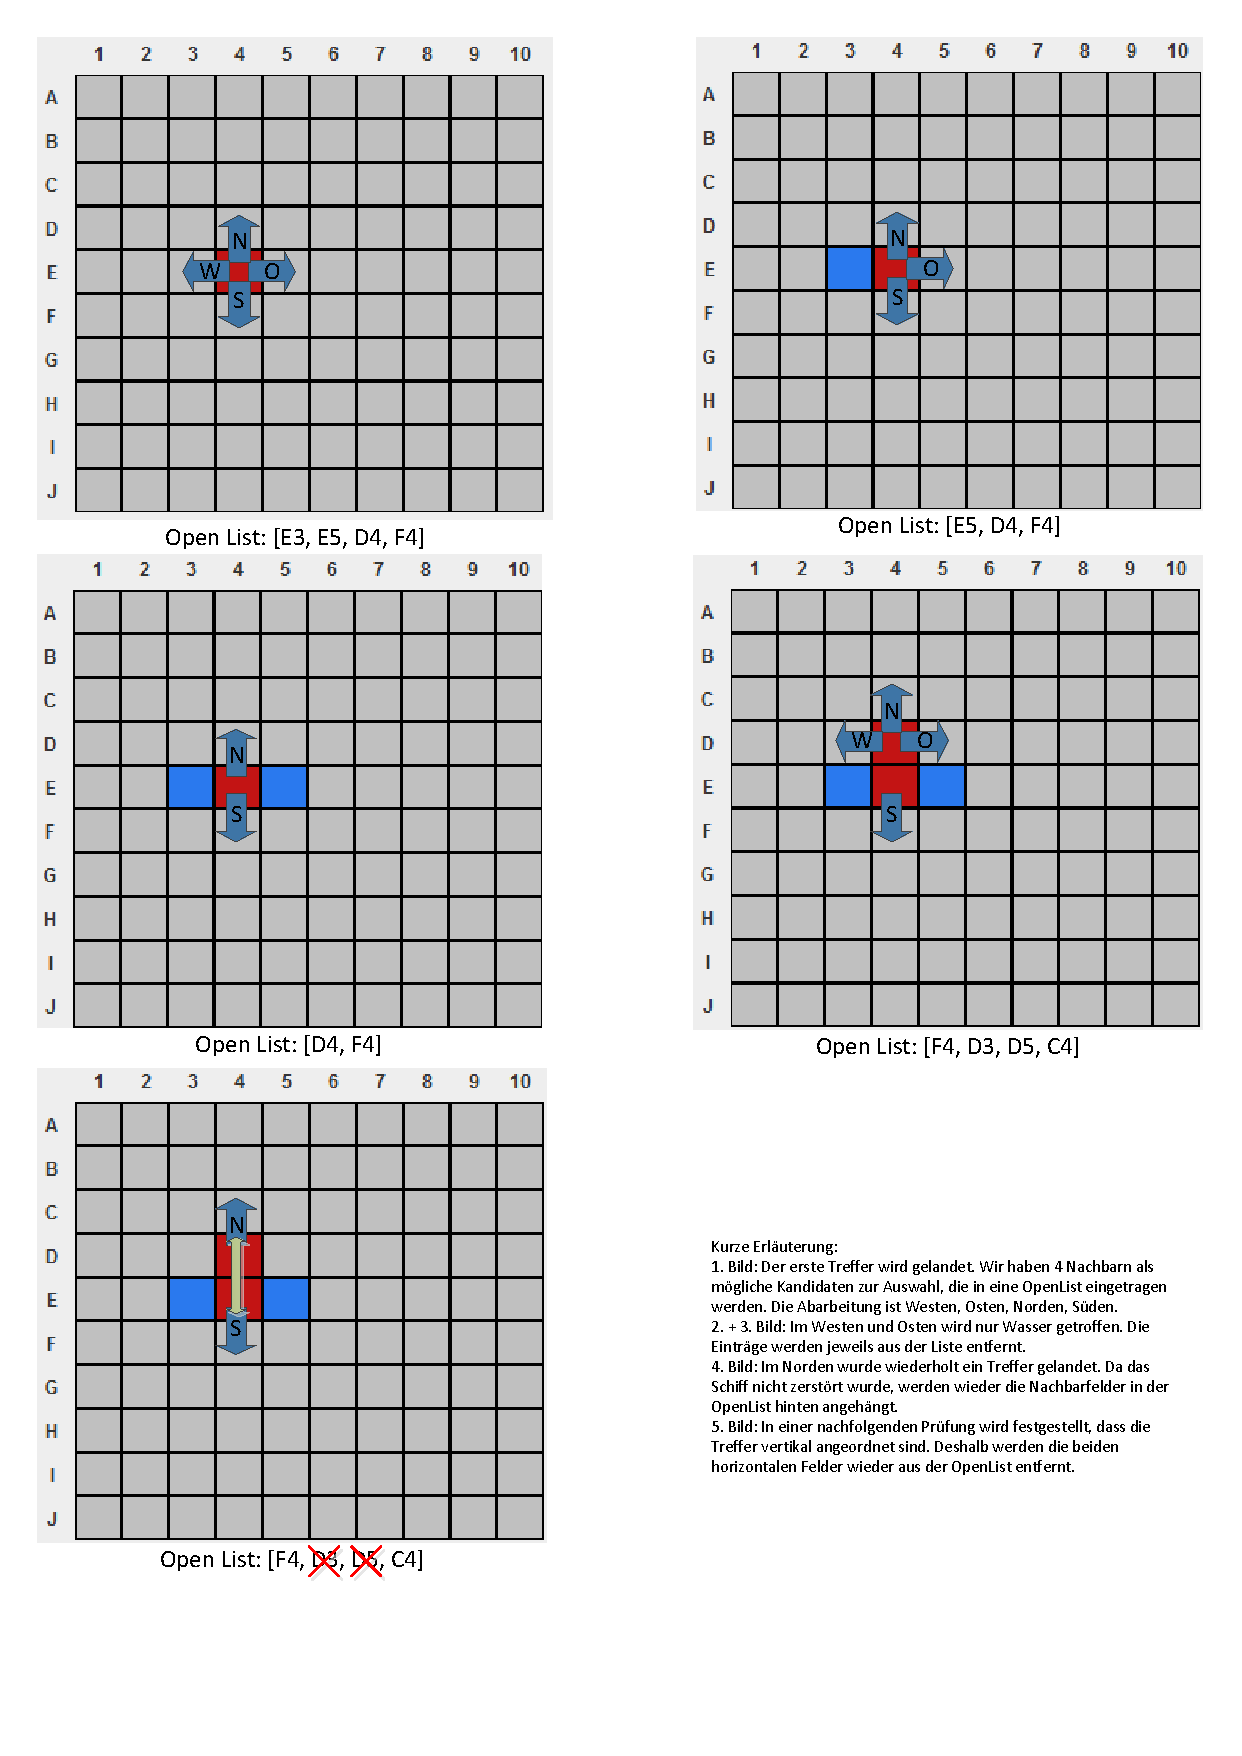
\includegraphics[trim=105mm 204mm 5mm 4mm,clip,width=0.47\textwidth]{images/Strategie_1_FirstHit.pdf}
    \label{fig:west}
  }
  \subfigure[Osten (verfehlt)]{
	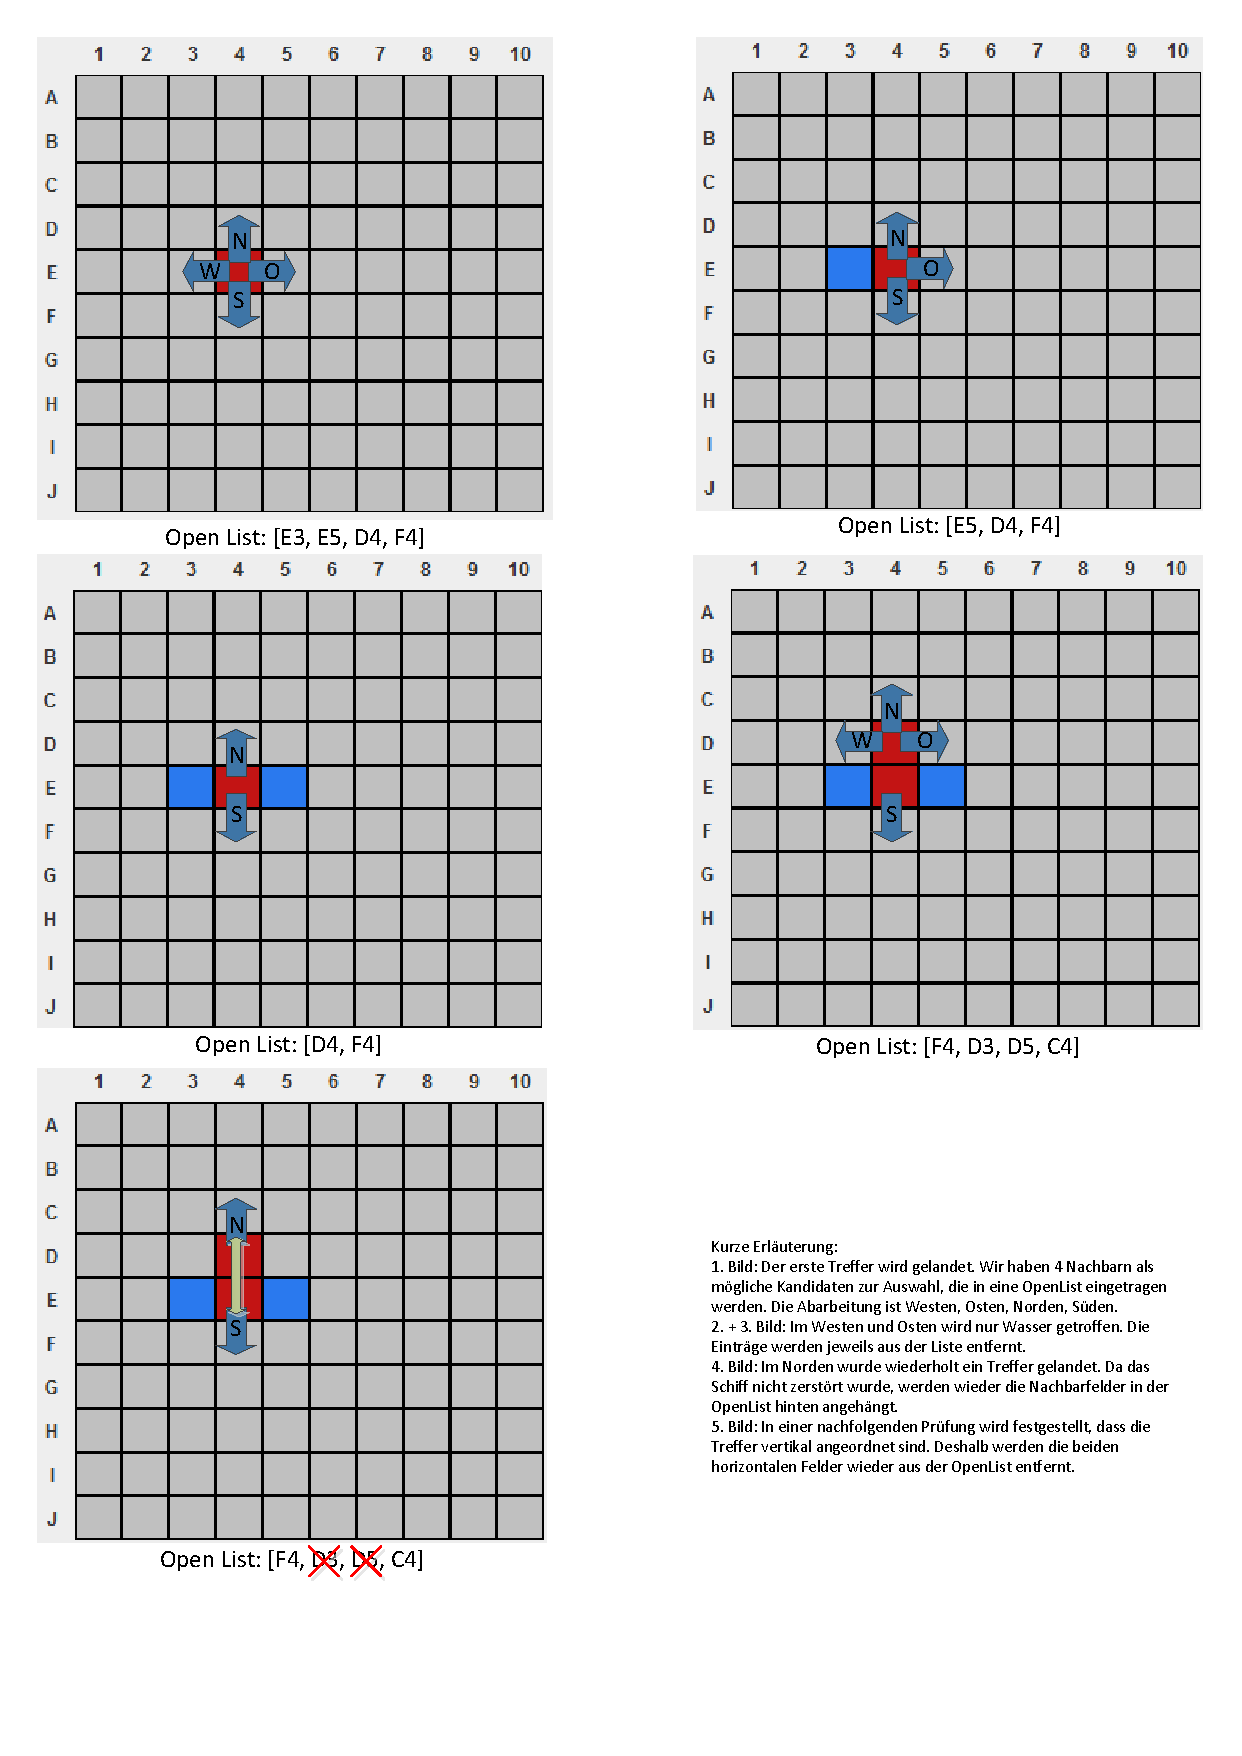
\includegraphics[trim=5mm 117mm 105mm 94mm,clip,width=0.47\textwidth]{images/Strategie_1_FirstHit.pdf}
    \label{fig:east}
  }
  \caption{Openlist nach zwei misglückten Angriffen}
  \label{fig:Openlist2}
\end{figure}

Im Falle eines weiteren Treffers wiederholt sich der Algorithmus und nimmt alle unbekannten und benachbarten Felder des Treffers in die Openlist auf (vgl. Abbilidung \ref{fig:north}).
Anschließend wird mit dem Prädikat \texttt{checkHitDirection/2} überprüft, ob die Orientierung des attackierten Schiffes (horizontal oder vertikal) bereits durch frühere Treffer bekannt ist. 
Ist dies der Fall, so kann die Openlist entsprechend um auszuschließende Positionen verkürzt werden.
Im hier gezeigten Beispiel können die horizontalen Felder $D3$ und $D5$ wieder aus der Liste gestrichen werden.
\begin{figure}[H]
  \centering
  \subfigure[Norden (Treffer)]{
    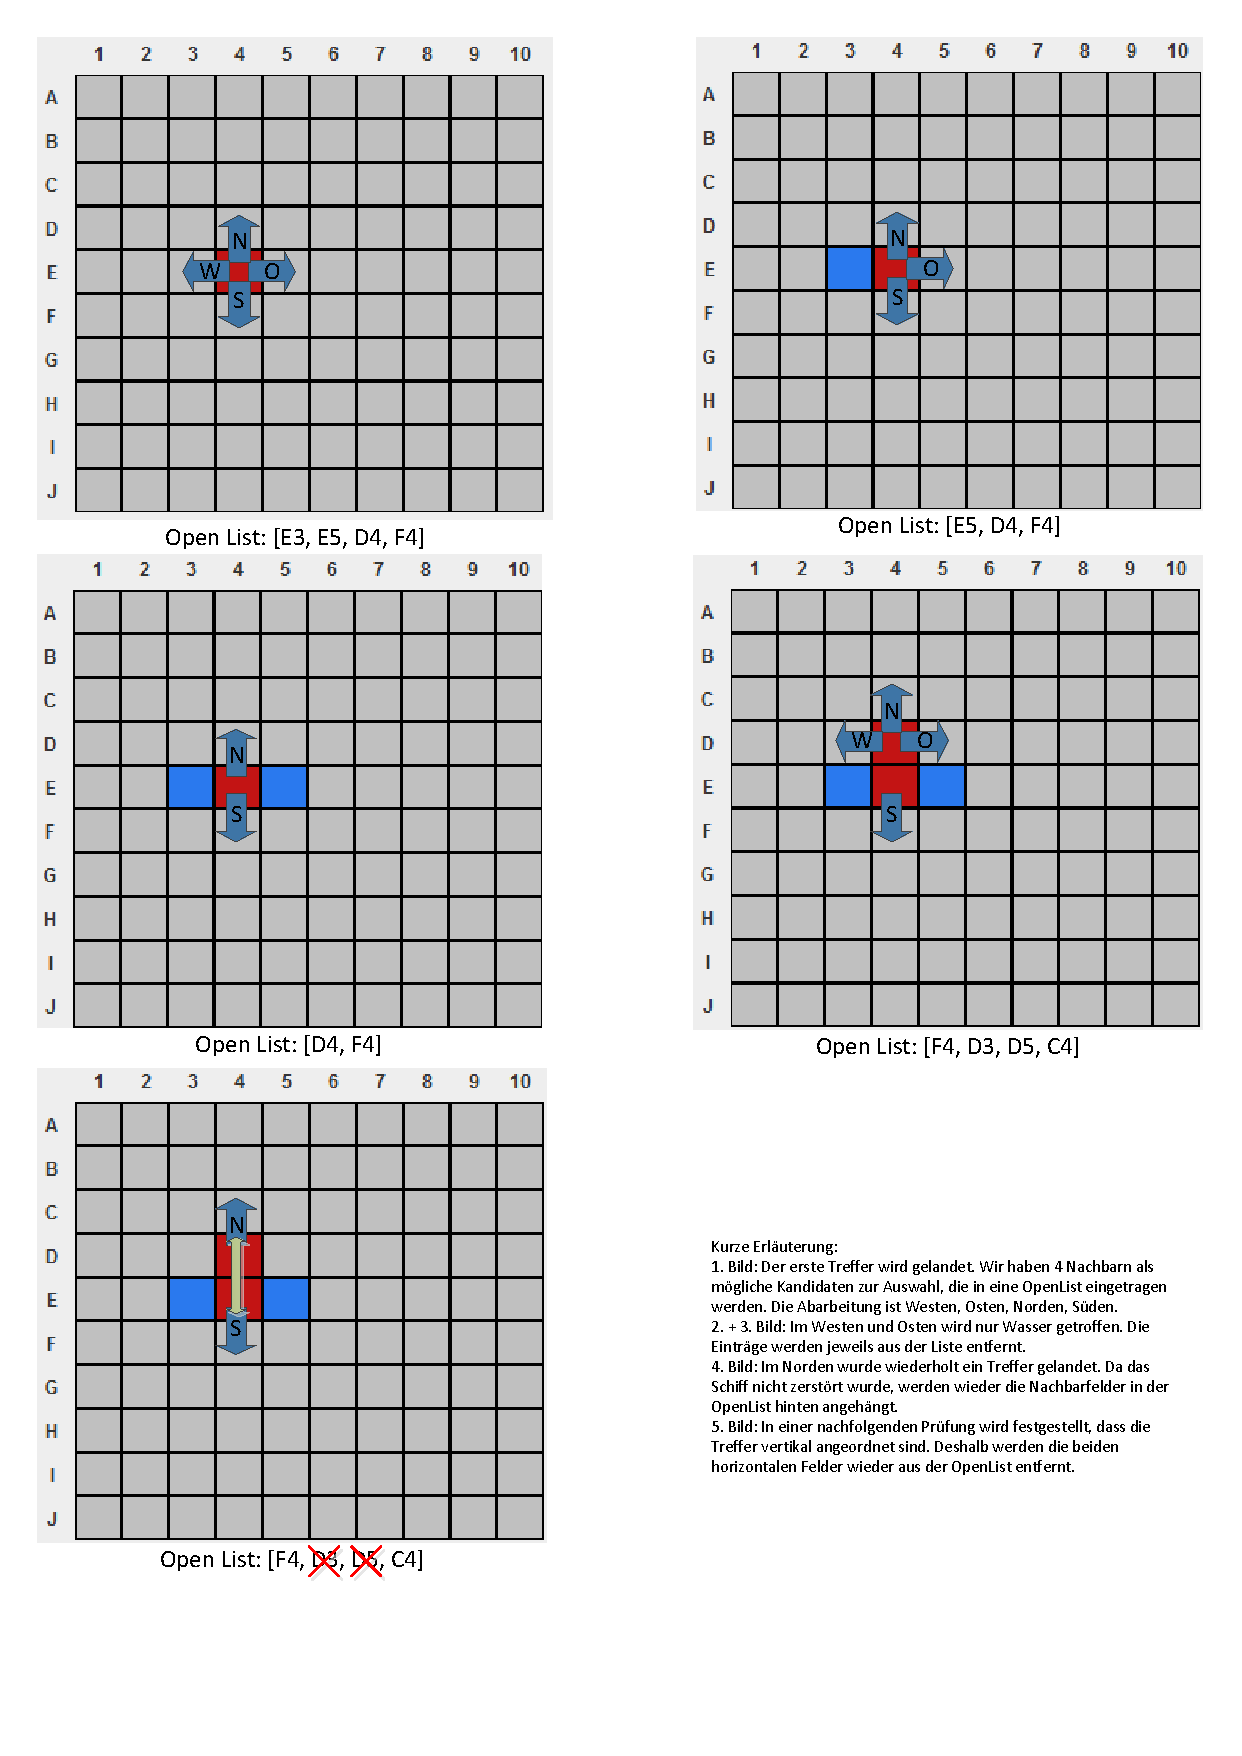
\includegraphics[trim=105mm 117mm 5mm 94mm,clip,width=0.47\textwidth]{images/Strategie_1_FirstHit.pdf}
    \label{fig:north}
  }
  \subfigure[Bereinigte Openlist]{
	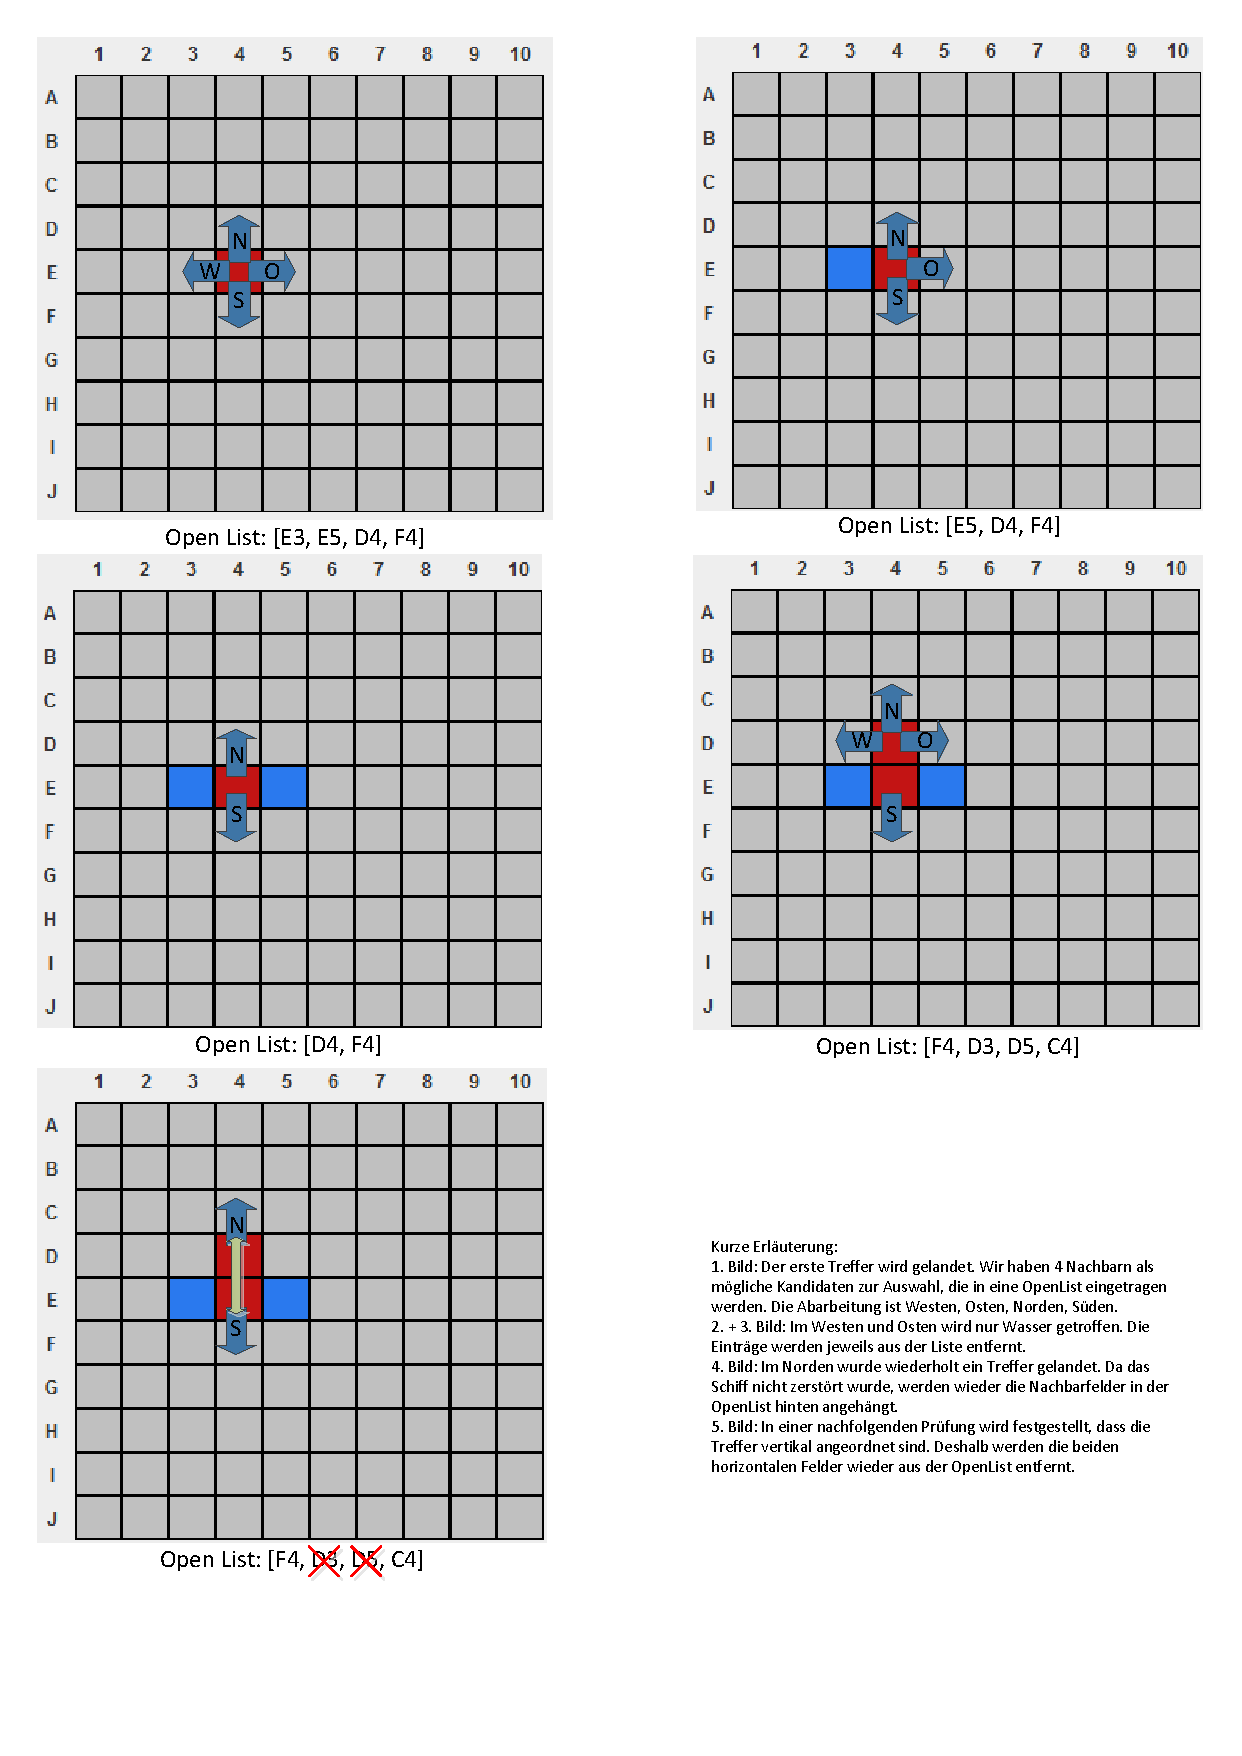
\includegraphics[trim=5mm 30mm 105mm 180mm,clip,width=0.47\textwidth]{images/Strategie_1_FirstHit.pdf}
    \label{fig:northupd}
  }
  \caption{Aktualisierung der Openlist nach einem Treffer}
  \label{fig:Openlist3}
\end{figure}

Nachdem das Schiff vollständig zerstört wurde, wird die Openlist geleert und die Auswahl der anzugreifenden Koordinaten erfolgt wieder solange zufällig, bis der nächste Treffer erzielt wurde.
% \subsubsection{Strategiemodul} \label{sec:strategy}

	% Das Strategiemodul \texttt{strategy.pl} stellt das Prädikat zur Bestimmung des nächsten Angriffspunktes \texttt{getPointOfAttack/2}
	% zur Verfügung. Außerdem füllt dieses Modul die Liste der priorisiert anzugreifenden Punkte über das Prädikat \texttt{updateOpenList/3}. 
	
	% Beim Aufruf von \texttt{getPointOfAttack/2} wird das erste Element der Openlist \texttt{openList/2} zurückgegeben.
	% Befinden sich keine Koordinaten in der Openlist \texttt{openList/1}, so gibt \texttt{getPointOfAttack/2} einen zufälligen Angriffspunkt zurück.
	
	% Das Prädikat \texttt{updateOpenList/3} erhält die angegriffene Koordinate und den vom Gegner erhaltenen Rückgabewert. 
	% Traf der Angriff Wasser oder das letzte Schiff des Gegners, so erfolgt keine Änderung der Openlist.
	
	% Wurde das gerade attackierte Schiff vollständig versenkt, so kann die aktuelle Openlist vollständig geleert werden, da stets nur ein 
	% Schiff attackiert wird. Außerdem werden die unmittelbar benachbarten Felder des versenkten Schiffes als \textit{Wasser} markiert, denn
	% Aufgrund der Spielregeln darf sich auf diesen Feldern kein weiteres Schiff befinden (Prädikat \texttt{surroundWithWater/4}). 
	
	% Ist die Antwort des Gegeners \textit{Treffer}, so muss die OpenList aktualisiert werden. 
	% Dazu werden zunächst alle benachbarten Felder in die Openlist eingetragen, deren Status unbekannt ist 
	% (Prädikat \texttt{appendFreeFieldToList/2}). 
	% Anschließend wird mit dem Prädikat \texttt{checkHitDirection/2} überprüft, ob die Orientierung 
	% des attackierten Schiffes (horizontal oder vertikal) bereits durch frühere Treffer bekannt ist. 
	% Ist dies der Fall, so kann die Openlist entsprechend um auszuschließende Positionen verkürzt werden.

\subsubsection{Ausgabemodul}
		Das Ausgabemodul \texttt{outputModule.pl} beinhaltet Prädikate zur Ausgabe der \textit{globalen Variablen} \texttt{myField/1},
		\texttt{enemyField/1} sowie \texttt{openList/1}. Die Ausgabe erfolgt standardgemäß auf der Standardausgabe und kann während des Spiels oder zu
		Debugzwecken verwendet werden.

		Um Eine Überflutung der Ausgabekonsole bei vielen automatisierten Spieldurchläufen (zum Beispiel: KI gegen KI, 1000 spiele) zu vermeiden, kann 
		die Ausgabe über das Prädikat \texttt{verbose/1} gesteuert werden (siehe Abschnitt \ref{ssub:ausgabeverhalten}).
\subsubsection{Ausgabeverhalten} % (fold)
\label{ssub:ausgabeverhalten}
\todoin{spellcheck??}
		Das Modul \texttt{verbosity.pl} steuert den Ausgabekanal, auf dem während des Spielens Debug-Informationen dargestellt werden können. 
		Es sind drei verschiedene Ausgabeverhalten implementiert:
			\begin{enumerate}
				\item \texttt{verbose(0)} : Keinerlei Ausgabe während des Spiels.
				\item \texttt{verbose(1)} : Ausgaben während des Spiels werden in eine Textdatei umgeleitet.
				\item \texttt{verbose(2)} : Ausgaben während des Spiels erscheinen auf der Konsole.
			\end{enumerate}
			Bei allen Modi wird nach Beendigung aller konfigurierten Spiele, eine Zusammenfassung der Ergebnisse (siehe Abschnitt \ref{subssec:hauptmodul}) 
			auf der Ausgabekonsole Ausgegeben.

			Zur Realisierung der verschiedenen Ausgabemodi wird der Standardausgabestrom der SWI-Prolog Umgebung über das Systemprädikat \texttt{set\_output/1} 
			geändert. Die Implementierung von \texttt{verbose/1} findet sich in \texttt{verbosity.pl}. Hier wird je nach Argument ein anderer Ausgabestrom 
			definiert und als Standardausgabestrom gesetzt:
			\begin{itemize}
				\item \texttt{verbose(0)} : erzeugen eines Null-Stroms per \texttt{open\_null\_stream/1}.
				\item \texttt{verbose(1)} : erzeugen eines Ausgabestroms in die Datei "'Output.txt"' im Unterordner "'GameLogs"' per \texttt{open/3}.
				\item \texttt{verbose(2)} : erzeugen eines Ausgabestroms auf die Ausgabekonsole per \texttt{user\_output/0}.
			\end{itemize}
			Nach dem erzeugen des jeweiligen Ausgabestroms wird dieser über das Systemprädikat \texttt{set\_output} gesetzt und der aktuelle Ausgabestrom 
			im globalen Prädikat \texttt{currentStream/1} gesetzt, sodass er überall im Programm manipuliert werden kann.
			Vor Ausgabe der Spielzusammenfassung wird der momentane Ausgabestrom über das oben beschriebene Prädikat \texttt{currentStream/1} geholt und 
			über das Systemprädikat \texttt{close/1} geschlossen. Direkt danach wird \texttt{verbose(2)} gesetzt, sodass die Ausgabe 
			der Zusammenfassung in jedem Fall auf der Ausgabekonsole erscheint.
% subsubsection ausgabeverhalten (end)
	


		\section{Evaluation} \label{sec:Evaluation}

\subsection{Testkonzept}
\todoin{Bogi, Vic - lest euch das bitte durch und guckt ob wir das wirklich so verteidigen können.. thx}

	Ziel der durchgeführten Tests war es, mögliche Fehlerzustände im implementierten Programm aufzudecken und außerdem zu belegen, dass das System
	wie erwartet funktioniert. 
	
	% White Box
	% \todoin{Entwicklertest, Testbarkeit der Software (Treiber,...), Positiv- und Negativtests,}
	Da die Verwendung strukturorientierter Testverfahren die Entwicklung eines Testrahmens bedeuten und dies den Rahmen des Projektes sprengen würde,
	wurde von der Verwendung dieser Verfahren abgesehen.  
	Stattdessen wurde der Einsatz verschiedener Black-Box Methoden vorgesehen.
	
	% Black Box
	% \subsection{Funktionaler Test}
	Um zu überprüfen ob das entwickelte Spiel die gewünschten Funktionen bietet, wurden funktionale Tests durchgeführt. 
	Als Spezifikation hierfür wurden die in Abschnitt \ref{sec:Spielregeln} beschriebenen Eigenschaften des Spiels \textit{Schiffe-Versenken}
	verwendet. 
	
	\todoin{zustandsbasierter test - testet auch ungültige zustandsübergänge - möglcih???}
	
	% nicht funktional
	Außerdem wurden auch nicht funktionale Testverfahren verwendet. In diesem Kontext wurde auch ein Langzeittest durchgeführt, bei dem zwei
	Prolog-Clients 1000 Spiele gegeneinander spielen. Ziel dieses Tests war es diese hohe Anzahl von Spielen fehlerfrei zu beenden. 	
	
	\todoin{nicht funktional: portabilitätstest - wurde ja auf 2 plattformen entwickelt??!}
	\todoin{nicht funktional: Benutzbarkeit - wurde von beate verifiziert ;) }

\subsection{Testfälle}
	Zur Umsetzung des beschriebenen Testkonzepts (siehe Abschnitt \ref{sec:Evaluation}) wurden konkrete Testfälle konzeptioniert und
	durchgeführt. Im Folgenden werden die Testfälle, ihre Durchführung und das Testergebnis beschrieben. 

	\subsubsection{Testfall 1, Testfall 2} % (fold)
	\label{ssub:testfall_1_testfall_2}
		Der erste Testfall untersucht die korrekte Initialisierung des Prologclients. Insbesondere stellt die regelkonforme Platzieung der
		Schiffe einen wichtigen Bestandteil des Spiels dar. 

		Im gleichen Rahmen der Prüfung auf die korrekte Platzierung der Schiffe muss ebenfalls validiert werden, ob die geforderte Anzahl an Schiffen und die
		korrekten Schiffstypen auf dem Spielfeld zu finden sind. Dies stellt den zweiten Testfall dar.
	
		Zur Überprüfung der Korrektheit der Platzierung, der richtigen Gesamtanzahl der Schiffe, sowie die korrekte Anzahl der einzelnen Typen, wurden 
		die Startaufstellungen von 100 KI-gegen-KI spielen gespeichert und ausgewertet. Bei jedem KI-gegen-KI Spiel erzeugt der Prolog Client zwei 
		Aufstellungen (eine je KI-Spieler). Die so resultierenden 200 Aufstellungen wurden vom Entwicklerteam ausgewertet und auf Korrektheit in den 
		angegebenen Aspekten überprüft.
		
		\paragraph{Testergebnis} % (fold)
		\label{par:testergebnis}
			Das Überprüfen der 200 generierten Aufstellungen ergab folgendes Ergebnis:
			\begin{table}[H] % (fold)
				\centering
				\begin{tabular}{|p{.15\textwidth}|p{.14\textwidth}|p{.13\textwidth}|p{.15\textwidth}|p{.15\textwidth}|p{.11\textwidth}|} 
					\hline
					Geprüfte\newline Aufstellungen & Fehlerhafte Platzierung&Fehlerhafte Anzahl&Fehlerhafte Typen&Korrekte\newline Aufstellungen&Duplikate\\ 
					\hline\hline
					200 & 0 & 0 & 0 & 200 & 0\\
					\hline
				\end{tabular}
				\caption{Testresultat für Testfall 1 und Testfall2}
				\label{tbl:tf1tf2}
			\end{table}
			% table tbl:tf1tf2 (end)
		% paragraph testergebnis (end)
		Das Testergebnis zeigt, dass die Routine zum Platzieren der Schiffe wie erwartet arbeitet. Beim Testen wurde gleichzeitig auch überprüft, 
		wie oft Duplikate durch die Routine erzeugt werden (also identische Platzierungen).
		Das Auftreten keiner Duplikate lässt schlussfolgern, dass der Einsatz der Prolog-Systemprädikate \texttt{random/1} und \texttt{randseq/3} 
		den gewünschten Effekt liefern (siehe Abschnitt \ref{sec:initships}) und wie erwartet arbeiten.
		
		Die Liste der Ausgewerteten Textdaten befindet sich in \newline \texttt{Battleship\textbackslash MyField\_200Testdaten.txt}
	% subsubsection testfall_1_testfall_2 (end)
	\subsubsection{Testfall 3} % (fold)
	\label{ssub:testfall_3}
	
	Der dritte Testfall behandelt die Auswahl des nächsten anzugreifenden Spielfeldes. Im besonderen Fokus steht die Aufgabe der Verfolgung eines 
	getroffenen, aber noch nicht versenkten Schiffes.
	Hierfür wurde ein Spieler-gegen-KI spiel durchgeführt und die Ausgaben der KI in eine Datei umgeleitet. Das Spiel wurde künstlich in die Länge 
	gezogen bis die KI gewann, indem der Spieler gezielt auf unbelegte Spielfelder der KI geschossen hat.
	Nachdem die KI gewann, wurde die mitgeschriebene Datei, analysiert. Hierbei wurden die von der KI ausgewählten zu attakierenden Felder gegen die,
	durch die Strategie (siehe Abschnitt \ref{sec:strategy}) zu erwartenden überprüft. Diese Analyse ist in Tabelle \ref{tbl:testfall3} nachzuvollziehen.
	\begin{table}[H] % (fold)
	\centering
	\begin{tabular}{|l|p{.2\textwidth}|p{.2\textwidth}|p{.15\textwidth}|p{.25\textwidth}|}
		\hline
		Nr.	&	beschossene Koordinate	&	verhalten Erwartungsgemäß	&	Antwort	&	Nächste zu erwartende Koordinate	\\
		\hline
		\hline
		0	&	-						& -								& -			& \emph{zufällig}						\\ \hline
		1	& 1 / 6						& \checkmark					& Wasser	& \emph{zufällig}						\\ \hline
		2	& 3 / 9						& \checkmark					& Treffer	& 2 / 9									\\ \hline
		3	& 2 / 9						& \checkmark					& Wasser	& 4 / 9									\\ \hline
		4	& 4 / 9						& \checkmark					& Treffer	& 5 / 9									\\ \hline
		5	& 5 / 9						& \checkmark					& \textbf{Versenkt}	& \emph{zufällig}						\\ \hline
		6	& 7 / 6						& \checkmark					& Wasser	& \emph{zufällig}						\\ \hline
		7	& 2 / 5						& \checkmark					& Wasser	& \emph{zufällig}						\\ \hline
		8	& 0 / 5						& \checkmark					& Wasser	& \emph{zufällig}						\\ \hline
		9	& 1 / 0						& \checkmark					& Wasser	& \emph{zufällig}						\\ \hline
		10	& 2 / 0						& \checkmark					& Treffer	& 3 / 0									\\ \hline
		11	& 3 / 0						& \checkmark					& Treffer	& 4 / 0									\\ \hline
		12	& 4 / 0						& \checkmark					& \textbf{Versenkt}	& \emph{zufällig}						\\ \hline
		13	& 8 / 1						& \checkmark					& Wasser	& \emph{zufällig}						\\ \hline
		14	& 2 / 3						& \checkmark					& Wasser	& \emph{zufällig}						\\ \hline
		15	& 3 / 6						& \checkmark					& Treffer	& 2 / 6									\\ \hline
		16	& 2 / 6						& \checkmark					& Wasser	& 4 / 6									\\ \hline
		17	& 4 / 6						& \checkmark					& Wasser	& 3 / 5									\\ \hline
		18	& 3 / 5						& \checkmark					& \textbf{Versenkt}	& \emph{zufällig}						\\ \hline
		19	& 1 / 9						& \checkmark					& Wasser	& \emph{zufällig}						\\ \hline
		20	& 5 / 2						& \checkmark					& Wasser	& \emph{zufällig}						\\ \hline
		21	& 2 / 4						& \checkmark					& Wasser	& \emph{zufällig}						\\ \hline
		22	& 6 / 1						& \checkmark					& Treffer	& 5 / 1									\\ \hline
		23	& 5 / 1						& \checkmark					& Wasser	& 7 / 1									\\ \hline
		24	& 7 / 1						& \checkmark					& Wasser	& 6 / 0									\\ \hline
		25	& 6 / 0						& \checkmark					& Wasser	& 6 / 2									\\ \hline
		26	& 6 / 2						& \checkmark					& Treffer	& 6 / 3									\\ \hline
		27	& 6 / 3						& \checkmark					& Treffer	& 6 / 4									\\ \hline
		28	& 6 / 4						& \checkmark					& \textbf{Versenkt}	& \emph{zufällig}						\\ \hline
		29	& 7 / 5						& \checkmark					& Wasser	& \emph{zufällig}						\\ \hline
		30	& 2 / 7						& \checkmark					& Wasser	& \emph{zufällig}						\\ \hline
		31	& 9 / 7						& \checkmark					& Wasser	& \emph{zufällig}						\\ \hline
		32	& 9 / 3						& \checkmark					& Treffer	& 8 / 3									\\ \hline
		33	& 8 / 3						& \checkmark					& Wasser	& 9 / 2									\\ \hline
		34	& 9 / 2						& \checkmark					& Treffer	& 9 / 4									\\ \hline
		35	& 9 / 4						& \checkmark					& Treffer	& 9 / 1									\\ \hline
		36	& 9 / 1						& \checkmark					& Wasser	& 9 / 5									\\ \hline
		37	& 9 / 5						& \checkmark					& Treffer	& 9 / 6									\\ \hline
		38	& 9 / 6						& \checkmark					& \textbf{Versenkt}	& \emph{\textbf{Spielende}}						\\ \hline
	\end{tabular}
	\caption{KI-Attacken entnommen aus \texttt{Gamelog1.txt}.}
	\label{tbl:testfall3}
\end{table}
% table tbl:testfall3 (end)
	
	\paragraph{Testergebnise} % (fold)
	\label{par:testergebnise}
	 \todoin {alles gut hier ...}
	% paragraph testergebnise (end)
	
	Der vierte Testfall untersucht die korrekte Behandlung eines versenkten Schiffes. Insbesondere soll geprüft werden, ob die Umgebung in einer 4er-Nachbarschaft
	mit Wasser aufgedeckt wird, da an diesen Stellen laut Regelbeschreibung keine Schiffe platziert werden dürfen und somit für die nachfolgenden Züge 
	uninteressant sind.
	\todoin{Beschreibung des Tests}
	
	Vorbedignung - KI Ausgabe auf der Konsole
	% subsubsection testfall_3 (end)
     \subsubsection{Unittest: CPlayingFieldController}
Die Controllerklasse \texttt{CPlayingFieldController} des Java-Clients wurde einem Unittest unterzogen.
Diese Klasse bildet das zentrale Element der Spiellogik.
Das Ziel dieses Tests ist die Sicherstellung der korrekten Statuswechsel, sowie die korrekte Repräsentation der Spielinformationen.

Jedoch ist eine Untersuchung der einzelnen Methoden in diesem Fall nicht zielführend, da die internen Zustände und Variablen nur durch den Nachrichtenaustausch indirekt manipuliert werden können.
Außerdem ist zu beachten, dass die Schiffsplatzierung zufällig erfolgt, sodass diese Komponente nicht vorhergesagt und somit geprüft werden kann.

Die Testsequenz entspricht den ersten Zügen eines angehenden Spiels. 
Sie unterteilt sich in die primär in die Phase der Initialisierung und die des laufenden Spiels.

Im Rahmen des Tests werden zwei Instanzen der Klasse \texttt{CPlayingFieldController} erzeugt, die sich mit dem Spieleserver verbinden.
Unmittelbar nachdem sich ein Client verbunden hat, geht dieser in die Initialisierungphase über, was anhand des Unittests bestätigt wurde.
Außerdem konnte ebenfalls bestätigt werden, dass der erste Spielteilnehmer erwartungemäß im Verteidigungszustand startet.

Im weiteren Verlauf der Testfolge verbindet sich ein zweiter Client.
Erwartungsgemäß konnte verifiziert werden, dass dieser zum Einen den ersten Angriff ausführt und zum Anderen in den \emph{RUNNING}-Status gewechselt ist.

In der zweiten Phase des Tests werden abwechselnd Angriffe gestartet und es wird geprüft, ob sich die internen Spielfelder den eingehenden Informationen entsprechend geändert haben.
Die korrekte Darstellung des gegnerischen Spielfelds von \emph{UNKNOWN} zu \emph{WATER} bzw. \emph{HIT} konnte bestätigt werden.

Nach zwei weiteren Spielzügen konnte der korrekte Wechsel vom Angriffs- in den Verteidigungszustand und vice versa verifiziert werden.

Da die Schiffe zufällig platziert werden, kann eine Evaluation des Spielendes nicht automatisch erfolgen.
Aus diesem Grund wurde händisch ein Spiel Java-Client vs. Java-Client ausgetragen und geprüft, ob nach dem letzten versenkten Schiff der entsprechende Statuswechsel erfolgte.
Auch dieser Test konnte erfolgreich bestätigt werden.
	%- eigene Schiffe gültig platziert
	%- richtige anzahl und größe der schiffe
	%- gegnerische schiffe werden attackiert wenn ein treffer gelandet wurde
	%- gegnerisches schiff wird nach versenken mit wasser umschlossen
	%- 
		
		\todoin{Benutzungshinweise für den Endbenutzer}
		\todoin{Ausblick - was fehlt noch? bekannte Fehler, spätere Verbesserungen, Fazit der Teilnehmer}
		\todoin{Ausblick: Überprüfung adden z.B. wenn 2er Versenkt, können alle 2er Lücken als Wasser markiert werden, etc.}
		\todoin{Ausblick: Schachbrettangriff}
		
		%!TEX root = /Users/stefanbogdanski/Dropbox/BÄTTLESHÖP/Dokumentation/dokumentation.text
%
% Apostel, Bogdanski, Ritter
%
% Wahlpflichtfach Künstliche Intelligenz:
% Projekt - Schiffe Versenken
%
% Hochschule Bremen - University of applied siences
% ============================================================================
%
% literatur.tex
%
% Beschreibung des Dateiinhalts

\nocite{*}
\bibliography{includes/thesis}
\bibliographystyle{is-abbrv}
		\let\cleardoublepage\clearpage
		\appendix
\end{document}                                                 
